%        File: arfc-beamer.tex
%     Created: Sun May 5 10:00 PM 2013 C


%\documentclass[11pt,handout]{beamer}
\documentclass[9pt]{beamer}
\usetheme[white]{Illinois}
%\title[short title]{long title}
\title[Research Summary]{Research Activities in the ARFC Group}
%\subtitle[short subtitle]{long subtitle}
\subtitle[Brief Summary]{A Brief Summary}
%\author[short name]{long name}
\author[ARFC]{Advanced Reactors and Fuel Cycles Group}
%\date[short date]{long date}
\date[09.05.2019]{September 5, 2019}
%\institution[short name]{long name}
\institute[UIUC]{University of Illinois at Urbana-Champaign}

%\usepackage{bbding}
\usepackage{amsfonts}
\usepackage{amsmath}
\usepackage{xspace}
\usepackage{graphicx}
\usepackage{subfigure}
\usepackage{booktabs} % nice rules for tables
\usepackage{microtype} % if using PDF
\usepackage{bigints}
\usepackage{minted}
\usepackage[absolute,overlay]{textpos}
\usepackage{tikz}
\usetikzlibrary{positioning, arrows, decorations, shapes}
\usetikzlibrary{shapes.geometric,arrows}
\definecolor{illiniblue}{HTML}{B1C6E2}
\tikzstyle{bblock} = [rectangle, draw, fill=illiniblue, 
text width=10em, text centered, rounded corners, minimum height=4em]
\tikzstyle{sbblock} = [rectangle, draw, fill=illiniblue, 
text width=7em, text centered, rounded corners, minimum height=4em]
\tikzstyle{arrow} = [thick,->,>=stealth]

\newcommand{\units}[1] {\:\text{#1}}%
\newcommand{\SN}{S$_N$}%{S$_\text{N}$}%{$S_N$}%
\DeclareMathOperator{\erf}{erf}
%I need some complimentary error funcitons... 
\DeclareMathOperator{\erfc}{erfc}
%Those icons in the references are terrible looking
\setbeamertemplate{bibliography item}[text]

%%%% Acronym support

\usepackage[acronym,toc]{glossaries}
%\newacronym{<++>}{<++>}{<++>}
\newacronym[longplural={metric tons of heavy metal}]{MTHM}{MTHM}{metric ton of heavy metal}
\newacronym{ABM}{ABM}{agent-based modeling}
\newacronym{ACDIS}{ACDIS}{Program in Arms Control \& Domestic and International Security}
\newacronym{AHTR}{AHTR}{Advanced High Temperature Reactor}
\newacronym{ANDRA}{ANDRA}{Agence Nationale pour la gestion des D\'echets RAdioactifs, the French National Agency for Radioactive Waste Management}
\newacronym{ANL}{ANL}{Argonne National Laboratory}
\newacronym{API}{API}{application programming interface}
\newacronym{ARE}{ARE}{Aircraft Reactor Experiment}
\newacronym{ARFC}{ARFC}{Advanced Reactors and Fuel Cycles}
\newacronym{ASME}{ASME}{American Society of Mechanical Engineers}
\newacronym{ATWS}{ATWS}{Anticipated Transient Without Scram}
\newacronym{BDBE}{BDBE}{Beyond Design Basis Event}
\newacronym{BIDS}{BIDS}{Berkeley Institute for Data Science}
\newacronym{CAFCA}{CAFCA}{ Code for Advanced Fuel Cycles Assessment }
\newacronym{CDTN}{CDTN}{Centro de Desenvolvimento da Tecnologia Nuclear}
\newacronym{CEA}{CEA}{Commissariat \`a l'\'Energie Atomique et aux \'Energies Alternatives}
\newacronym{CI}{CI}{continuous integration}
\newacronym{CNEN}{CNEN}{Comiss\~{a}o Nacional de Energia Nuclear}
\newacronym{CNERG}{CNERG}{Computational Nuclear Engineering Research Group}
\newacronym{COSI}{COSI}{Commelini-Sicard}
\newacronym{COTS}{COTS}{commercial, off-the-shelf}
\newacronym{CSNF}{CSNF}{commercial spent nuclear fuel}
\newacronym{CTAH}{CTAHs}{Coiled Tube Air Heaters}
\newacronym{CUBIT}{CUBIT}{CUBIT Geometry and Mesh Generation Toolkit}
\newacronym{CURIE}{CURIE}{Centralized Used Fuel Resource for Information Exchange}
\newacronym{DAG}{DAG}{directed acyclic graph}
\newacronym{DANESS}{DANESS}{Dynamic Analysis of Nuclear Energy System Strategies}
\newacronym{DBE}{DBE}{Design Basis Event}
\newacronym{DESAE}{DESAE}{Dynamic Analysis of Nuclear Energy Systems Strategies}
\newacronym{DHS}{DHS}{Department of Homeland Security}
\newacronym{DOE}{DOE}{Department of Energy}
\newacronym{DRACS}{DRACS}{Direct Reactor Auxiliary Cooling System}
\newacronym{DRE}{DRE}{dynamic resource exchange}
\newacronym{DSNF}{DSNF}{DOE spent nuclear fuel}
\newacronym{DYMOND}{DYMOND}{Dynamic Model of Nuclear Development }
\newacronym{EBS}{EBS}{Engineered Barrier System}
\newacronym{EDZ}{EDZ}{Excavation Disturbed Zone}
\newacronym{EIA}{EIA}{U.S. Energy Information Administration}
\newacronym{EPA}{EPA}{Environmental Protection Agency}
\newacronym{EP}{EP}{Engineering Physics}
\newacronym{FCO}{FCO}{Fuel Cycle Options}
\newacronym{FCT}{FCT}{Fuel Cycle Technology}
\newacronym{FEHM}{FEHM}{Finite Element Heat and Mass Transfer}
\newacronym{FEPs}{FEPs}{Features, Events, and Processes}
\newacronym{FHR}{FHR}{Fluoride-Salt-Cooled High-Temperature Reactor}
\newacronym{FLiBe}{FLiBe}{Fluoride-Lithium-Beryllium}
\newacronym{GDSE}{GDSE}{Generic Disposal System Environment}
\newacronym{GDSM}{GDSM}{Generic Disposal System Model}
\newacronym{GENIUSv1}{GENIUSv1}{Global Evaluation of Nuclear Infrastructure Utilization Scenarios, Version 1}
\newacronym{GENIUSv2}{GENIUSv2}{Global Evaluation of Nuclear Infrastructure Utilization Scenarios, Version 2}
\newacronym{GENIUS}{GENIUS}{Global Evaluation of Nuclear Infrastructure Utilization Scenarios}
\newacronym{GPAM}{GPAM}{Generic Performance Assessment Model}
\newacronym{GRSAC}{GRSAC}{Graphite Reactor Severe Accident Code}
\newacronym{GUI}{GUI}{graphical user interface}
\newacronym{HLW}{HLW}{high level waste}
\newacronym{HPC}{HPC}{high-performance computing}
\newacronym{HTC}{HTC}{high-throughput computing}
\newacronym{HTGR}{HTGR}{High Temperature Gas-Cooled Reactor}
\newacronym{IAEA}{IAEA}{International Atomic Energy Agency}
\newacronym{IEMA}{IEMA}{Illinois Emergency Mangament Agency}
\newacronym{INL}{INL}{Idaho National Laboratory}
\newacronym{IPRR1}{IRP-R1}{Instituto de Pesquisas Radioativas Reator 1}
\newacronym{IRP}{IRP}{Integrated Research Project}
\newacronym{ISFSI}{ISFSI}{Independent Spent Fuel Storage Installation}
\newacronym{ISRG}{ISRG}{Independent Student Research Group}
\newacronym{JFNK}{JFNK}{Jacobian-Free Newton Krylov}
\newacronym{LANL}{LANL}{Los Alamos National Laboratory}
\newacronym{LBNL}{LBNL}{Lawrence Berkeley National Laboratory}
\newacronym{LCOE}{LCOE}{levelized cost of electricity}
\newacronym{LDRD}{LDRD}{laboratory directed research and development}
\newacronym{LFR}{LFR}{Lead-Cooled Fast Reactor}
\newacronym{LLNL}{LLNL}{Lawrence Livermore National Laboratory}
\newacronym{LMFBR}{LMFBR}{Liquid Metal Fast Breeder Reactor}
\newacronym{LOFC}{LOFC}{Loss of Forced Cooling}
\newacronym{LOHS}{LOHS}{Loss of Heat Sink}
\newacronym{LOLA}{LOLA}{Loss of Large Area}
\newacronym{LP}{LP}{linear program}
\newacronym{MA}{MA}{minor actinide}
\newacronym{MCNP}{MCNP}{Monte Carlo N-Particle code}
\newacronym{MILP}{MILP}{mixed-integer linear program}
\newacronym{MIT}{MIT}{the Massachusetts Institute of Technology}
\newacronym{MOAB}{MOAB}{Mesh-Oriented datABase}
\newacronym{MOOSE}{MOOSE}{Multiphysics Object-Oriented Simulation Environment}
\newacronym{MOX}{MOX}{mixed oxide}
\newacronym{MSBR}{MSBR}{Molten Salt Breeder Reactor}
\newacronym{MSFR}{MSFR}{Molten Salt Fast Reactor}
\newacronym{MSRE}{MSRE}{Molten Salt Reactor Experiment}
\newacronym{MSR}{MSR}{Molten Salt Reactor}
\newacronym{NAGRA}{NAGRA}{National Cooperative for the Disposal of Radioactive Waste}
\newacronym{NEAMS}{NEAMS}{Nuclear Engineering Advanced Modeling and Simulation}
\newacronym{NEUP}{NEUP}{Nuclear Energy University Programs}
\newacronym{NFCSim}{NFCSim}{Nuclear Fuel Cycle Simulator}
\newacronym{NGNP}{NGNP}{Next Generation Nuclear Plant}
\newacronym{NMWPC}{NMWPC}{Nuclear MW Per Capita}
\newacronym{NNSA}{NNSA}{National Nuclear Security Administration}
\newacronym{NPRE}{NPRE}{Department of Nuclear, Plasma, and Radiological Engineering}
\newacronym{NQA1}{NQA-1}{Nuclear Quality Assurance - 1}
\newacronym{NRC}{NRC}{Nuclear Regulatory Commission}
\newacronym{NSF}{NSF}{National Science Foundation}
\newacronym{NSSC}{NSSC}{Nuclear Science and Security Consortium}
\newacronym{NUWASTE}{NUWASTE}{Nuclear Waste Assessment System for Technical Evaluation}
\newacronym{NWF}{NWF}{Nuclear Waste Fund}
\newacronym{NWTRB}{NWTRB}{Nuclear Waste Technical Review Board}
\newacronym{OCRWM}{OCRWM}{Office of Civilian Radioactive Waste Management}
\newacronym{ORION}{ORION}{ORION}
\newacronym{ORNL}{ORNL}{Oak Ridge National Laboratory}
\newacronym{PARCS}{PARCS}{Purdue Advanced Reactor Core Simulator}
\newacronym{PBAHTR}{PB-AHTR}{Pebble Bed Advanced High Temperature Reactor}
\newacronym{PBFHR}{PB-FHR}{Pebble-Bed Fluoride-Salt-Cooled High-Temperature Reactor}
\newacronym{PEI}{PEI}{Peak Environmental Impact}
\newacronym{PH}{PRONGHORN}{PRONGHORN}
\newacronym{PRKE}{PRKE}{Point Reactor Kinetics Equations}
\newacronym{PSPG}{PSPG}{Pressure-Stabilizing/Petrov-Galerkin}
\newacronym{PWAR}{PWAR}{Pratt and Whitney Aircraft Reactor}
\newacronym{PWR}{PWR}{Pressurized Water Reactor}
\newacronym{PyNE}{PyNE}{Python toolkit for Nuclear Engineering}
\newacronym{PyRK}{PyRK}{Python for Reactor Kinetics}
\newacronym{QA}{QA}{quality assurance}
\newacronym{RDD}{RD\&D}{Research Development and Demonstration}
\newacronym{RD}{R\&D}{Research and Development}
\newacronym{RELAP}{RELAP}{Reactor Excursion and Leak Analysis Program}
\newacronym{RIA}{RIA}{Reactivity Insertion Accident}
\newacronym{RIF}{RIF}{Region-Institution-Facility}
\newacronym{SFR}{SFR}{Sodium-Cooled Fast Reactor}
\newacronym{SINDAG}{SINDA{\textbackslash}G}{Systems Improved Numerical Differencing Analyzer $\backslash$ Gaski}
\newacronym{SKB}{SKB}{Svensk K\"{a}rnbr\"{a}nslehantering AB}
\newacronym{SNF}{SNF}{spent nuclear fuel}
\newacronym{SNL}{SNL}{Sandia National Laboratory}
\newacronym{STC}{STC}{specific temperature change}
\newacronym{SUPG}{SUPG}{Streamline-Upwind/Petrov-Galerkin}
\newacronym{SWF}{SWF}{Separations and Waste Forms}
\newacronym{SWU}{SWU}{Separative Work Unit}
\newacronym{TRIGA}{TRIGA}{Training Research Isotope General Atomic}
\newacronym{TRISO}{TRISO}{Tristructural Isotropic}
\newacronym{TSM}{TSM}{Total System Model}
\newacronym{TSPA}{TSPA}{Total System Performance Assessment for the Yucca Mountain License Application}
\newacronym{ThOX}{ThOX}{thorium oxide}
\newacronym{UFD}{UFD}{Used Fuel Disposition}
\newacronym{UML}{UML}{Unified Modeling Language}
\newacronym{UOX}{UOX}{uranium oxide}
\newacronym{UQ}{UQ}{uncertainty quantification}
\newacronym{US}{US}{United States}
\newacronym{UW}{UW}{University of Wisconsin}
\newacronym{VISION}{VISION}{the Verifiable Fuel Cycle Simulation Model}
\newacronym{VV}{V\&V}{verification and validation}
\newacronym{WIPP}{WIPP}{Waste Isolation Pilot Plant}
\newacronym{YMR}{YMR}{Yucca Mountain Repository Site}


\makeglossaries

%try to get rid of header on title page\dots
\makeatletter
    \newenvironment{withoutheadline}{
        \setbeamertemplate{headline}[default]
        \def\beamer@entrycode{\vspace*{-\headheight}}
    }{}
\makeatother

\makeatother
\setbeamertemplate{footline}
{
  \leavevmode%
  \hbox{%
    \rightline{\insertframenumber{} / \inserttotalframenumber\hspace*{1ex}}
  }%
  \vskip0pt%
}
\makeatletter
\begin{document}
%%%%%%%%%%%%%%%%%%%%%%%%%%%%%%%%%%%%%%%%%%%%%%%%%%%%%%%%%%%%%
%% From uw-beamer Here's a handy bit of code to place at 
%% the beginning of your presentation (after \begin{document}):
\newcommand*{\alphabet}{ABCDEFGHIJKLMNOPQRSTUVWXYZabcdefghijklmnopqrstuvwxyz}
\newlength{\highlightheight}
\newlength{\highlightdepth}
\newlength{\highlightmargin}
\setlength{\highlightmargin}{2pt}
\settoheight{\highlightheight}{\alphabet}
\settodepth{\highlightdepth}{\alphabet}
\addtolength{\highlightheight}{\highlightmargin}
\addtolength{\highlightdepth}{\highlightmargin}
\addtolength{\highlightheight}{\highlightdepth}
\newcommand*{\Highlight}{\rlap{\textcolor{HighlightBackground}{\rule[-\highlightdepth]{\linewidth}{\highlightheight}}}}
%%%%%%%%%%%%%%%%%%%%%%%%%%%%%%%%%%%%%%%%%%%%%%%%%%%%%%%%%%%%%
%%--------------------------------%%
\begin{withoutheadline}
\frame{
  \titlepage
}
\end{withoutheadline}

%%--------------------------------%%
\AtBeginSection[]{
\begin{frame}
  \frametitle{Outline}
  \tableofcontents[currentsection]
\end{frame}
}

\section{Software}
\begin{frame}
\frametitle{Cyclus}
\begin{block}{What is Cyclus?}
	Cyclus is a modular agent based fuel cycle simulator for tracking commodity transactions
	between facilities.
\end{block}
\begin{figure}
	\centering
	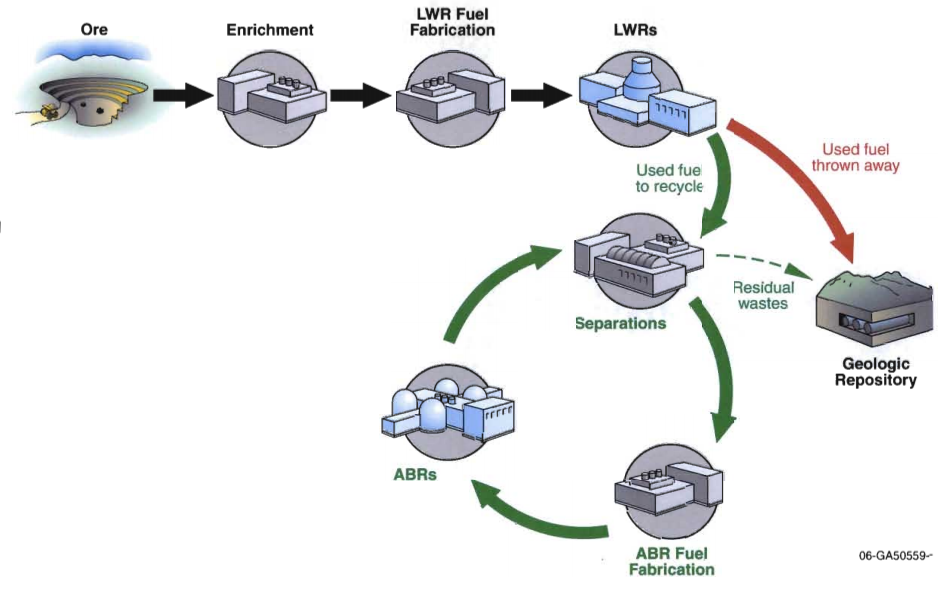
\includegraphics[width=0.7\linewidth]{./images/lanl-fuel-cycle.png}
	\label{fig:fuelcycle}
\end{figure}
\end{frame}

\begin{frame}
\frametitle{Why Cyclus?}
Cyclus allows the construction of specific scenarios through the addition of archetypes. These archetypes are
modular and the transactions can be tracked.
	\begin{figure}
		\centering
		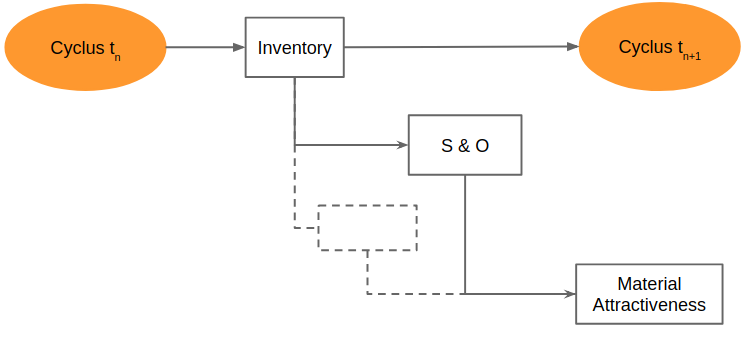
\includegraphics[width=0.9\linewidth]{./images/diversion1}
		\caption{Material transactions within Cyclus.}
		\label{fig:transactions}
	\end{figure}
\end{frame}
\begin{frame}
	\frametitle{Moltres}
	\begin{columns}
		\column[t]{5cm}
		\begin{itemize}
			\item Moltres is an application code built on the \gls{MOOSE}
			framework, for the simulation of \glspl{MSR}.
			\item MOOSE is an open source finite element framework that
			relies on libMesh and PETSc for their advanced meshing and PDE
			solver capabilities.
			\item MOOSE provides a simple interface for creating application
			codes for simulating various physical phenomena.
			\item Moltres can run transient, fully implicit coupled
			neutronics/thermal-hydraulics simulations of \glspl{MSR}.
		\end{itemize}
		\column[t]{5cm}
%		\begin{figure}
%			\centering
%			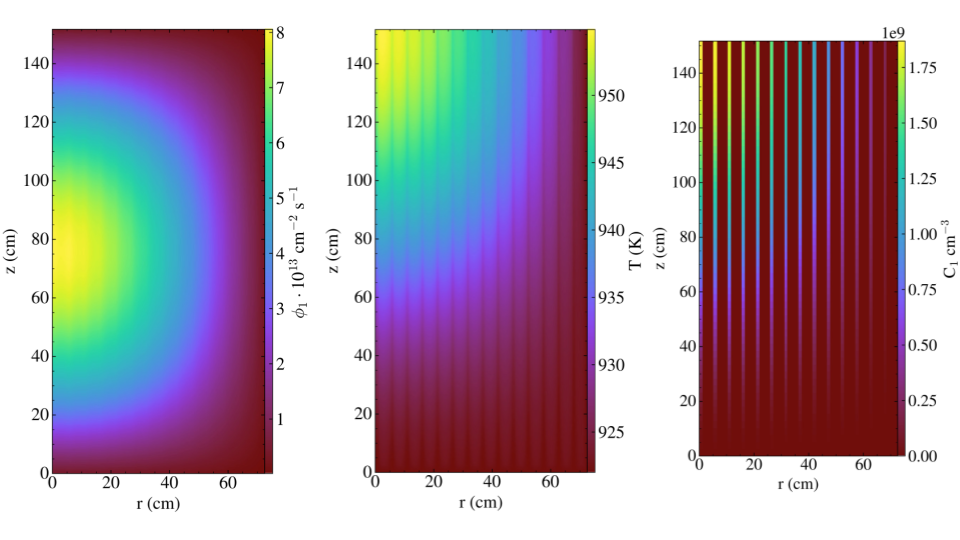
\includegraphics[width=.9\textwidth]{./images/msre}
%		\end{figure}
\end{frame}
\begin{frame}
\frametitle{SaltProc flowchart}
\vspace{-2mm}
\begin{figure}[ht!] % replace 't' with 'b' to \centering
	\centering
	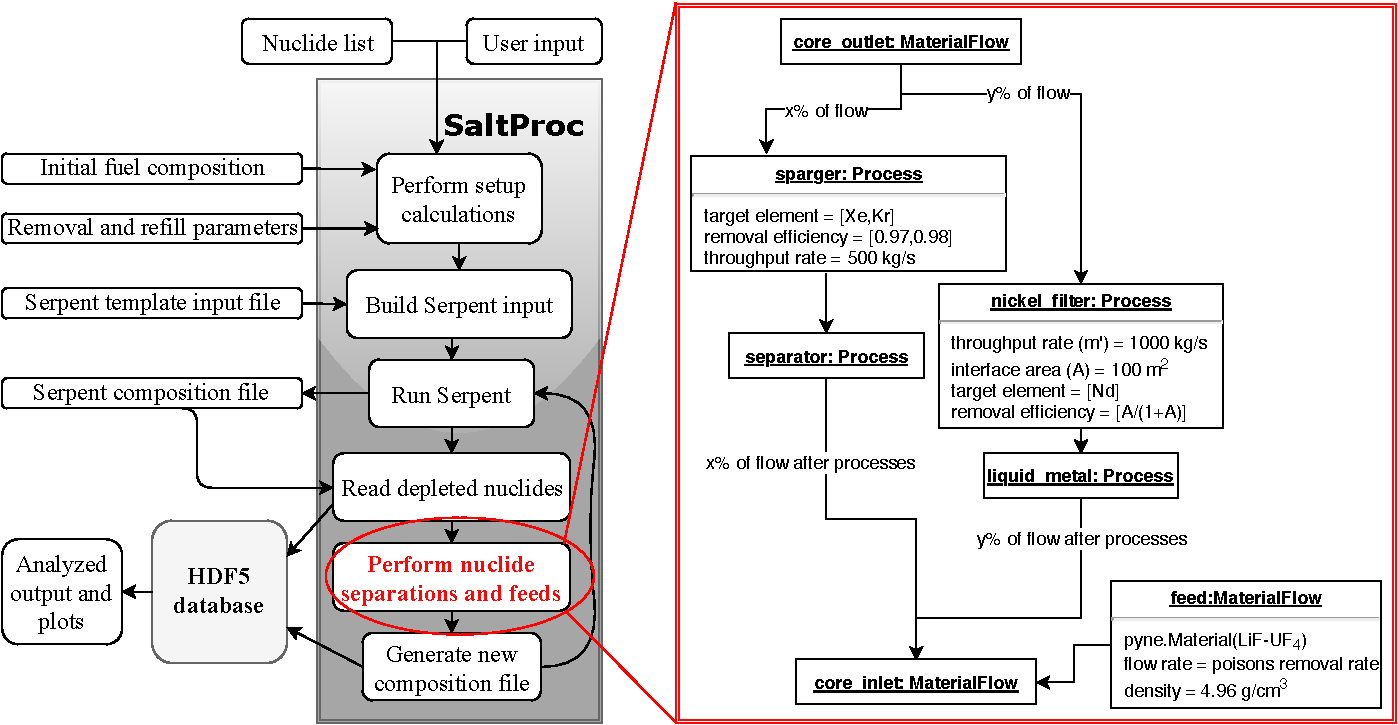
\includegraphics[width=1.05\textwidth]{./images/saltproc_flowchart.pdf}
	\caption{Tentative generic flowchart for SaltProc v1.0 python package.}
\end{figure}

\end{frame}
\input{annsa}
\documentclass{beamer}
% \usetheme{Illinois}
\usecolortheme{IllinoisWhite}

\usepackage{graphicx}
\graphicspath{{./images/}}

\title{Machine Learning Applications in Nuclear Engineering}
\author{Sam Dotson}
\institute{University of Illinois at Urbana-Champaign}
\date{2019}

\begin{document}
\frame{\titlepage}
	\begin{frame}
		\frametitle{Table of Contents}
		\tableofcontents
	\end{frame}

	\section{ANNSA}

	\begin{frame}
		\frametitle{\texttt{ANNSA}}
		``$\textbf{A}$rtificial $\textbf{N}$eural $\textbf{N}$etworks for $\textbf{S}$pectroscopic $\textbf{A}$nalysis"\\
		\begin{enumerate}
			\item Isotopics
			\item Nuclear Verification
			\item National Security 
			\item Machine Learning
		\end{enumerate}
	\end{frame}	
	\begin{frame}
		\frametitle{$\texttt{ANNSA}$}
		\begin{enumerate}
			\item Motivation\\
			Improve upon the current spectroscopy workflow
			\item Method\\
			Convolutional Neural Networks
		\end{enumerate} 
	\end{frame}
	% image frame
	\begin{frame}
		\frametitle{$\texttt{ANNSA}$ - Convolutional Neural Network}
		\begin{figure}
			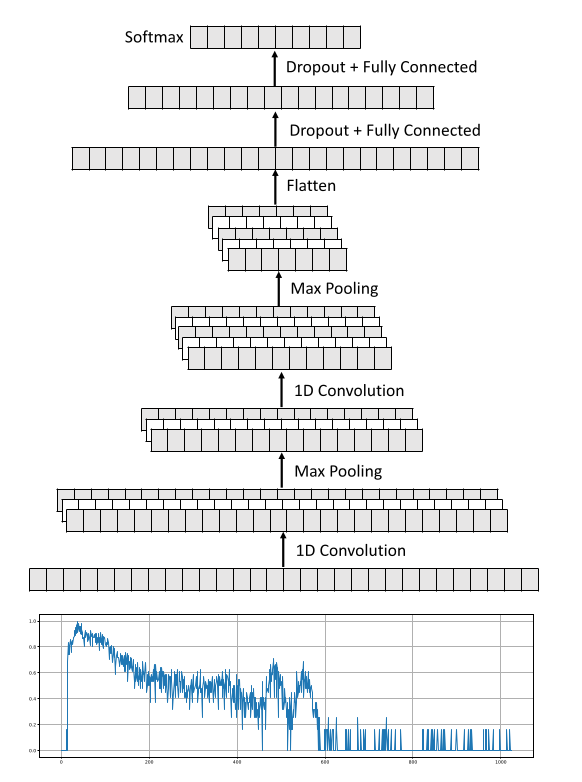
\includegraphics[width=5cm]{cnn-figure.png}
			\caption{Credit goes to Mark Kamuda}
		\end{figure}
	\end{frame}

	\begin{frame}
		\frametitle{$\texttt{ANNSA}$ - Extensions and Future Work}
		\begin{enumerate}
			\item Algorithm Improvements
			\item Different Detectors
			\item More complicated isotopics
		\end{enumerate}
	\end{frame}

	\section{CAIRO}

	\begin{frame}
		\frametitle{\texttt{CAIRO}}
		``$\textbf{C}$omputerized $\textbf{A}$rtificially $\textbf{I}$ntelligent $\textbf{R}$eactor $\textbf{O}$perator"\\
		\begin{enumerate}
			\item Nuclear Power
			\item Reactor Controls
			\item Control Room Simulation
			\item Artificial Intelligence
		\end{enumerate}
	\end{frame}

	\begin{frame}
		\frametitle{CAIRO - Motivation}
		\begin{figure}
			
\includegraphics[width=5cm]{homer-reactor.jpg}
		\end{figure}
	\end{frame}
	\begin{frame}
		\frametitle{CAIRO - Current Work}
		\begin{enumerate}
			\item Microreactor control room simulator
			\begin{enumerate}
				\item Core
				\item Electricity generator
				\item Control room interface
			\end{enumerate}
			\item Best representation of nuclear power plant for a deep reinforcement learning agent?
			\item What is an appropriate reward function(s) for a deep RL agent?
			\item Much more... 
		\end{enumerate}
	\end{frame}



\end{document}
\section{Advanced Reactors}
\begin{frame}
	\frametitle{Sun Myung Park: Coupled neutronics/thermal-hydraulics analysis}
		\begin{columns}
		\column[t]{6cm}
		My current research interests:
		\begin{block}{Moltres}
			\begin{itemize}
				\item Developing and improving capabilities in Moltres \\
				\item Currently working on
				implementing the k-$\epsilon$ turbulence model in Moltres.
			\end{itemize}
		\end{block}
		\begin{block}{\gls{MSFR}}
			\begin{itemize}
			\item Performing safety analyses of the \gls{MSFR} for various
			accident transients using Moltres with the k-$\epsilon$ model to
			include turbulence effects
			\end{itemize}
		\end{block}
		\column[t]{4cm}
		\begin{figure}[htbp!]
			\begin{center}
				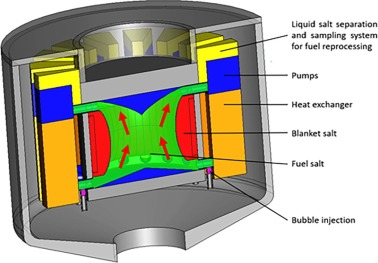
\includegraphics[height=3cm]{./images/msfr}
			\end{center}
			\caption{Schematic diagram of the \gls{MSFR}}
			\label{fig:msfr}
		\end{figure}
		\end{columns}
\end{frame}

\begin{frame}
	\frametitle{Sun Myung Park}
		\begin{columns}
			\column[t]{.5\textwidth}
			\begin{figure}[htbp!]
				\centering
				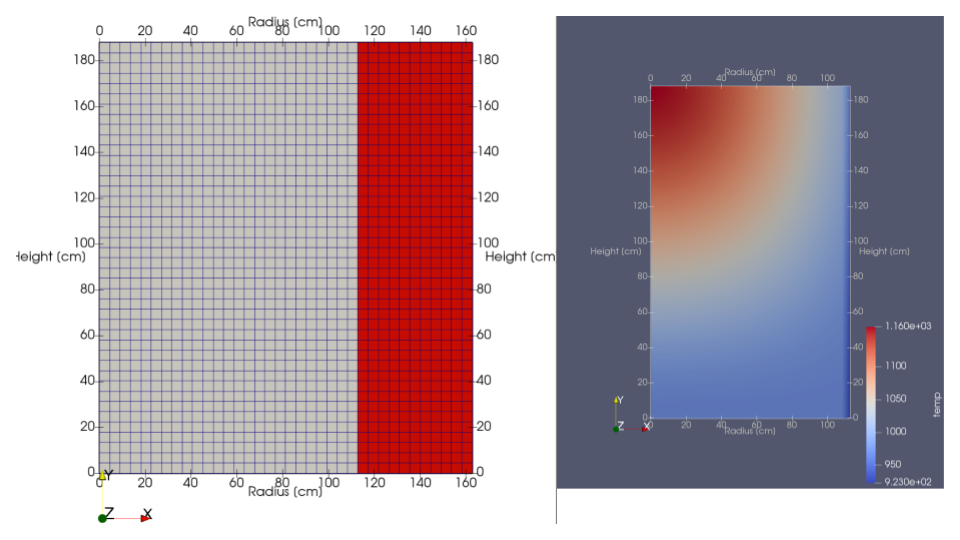
\includegraphics[height=2.8cm]{./images/mesh}
      			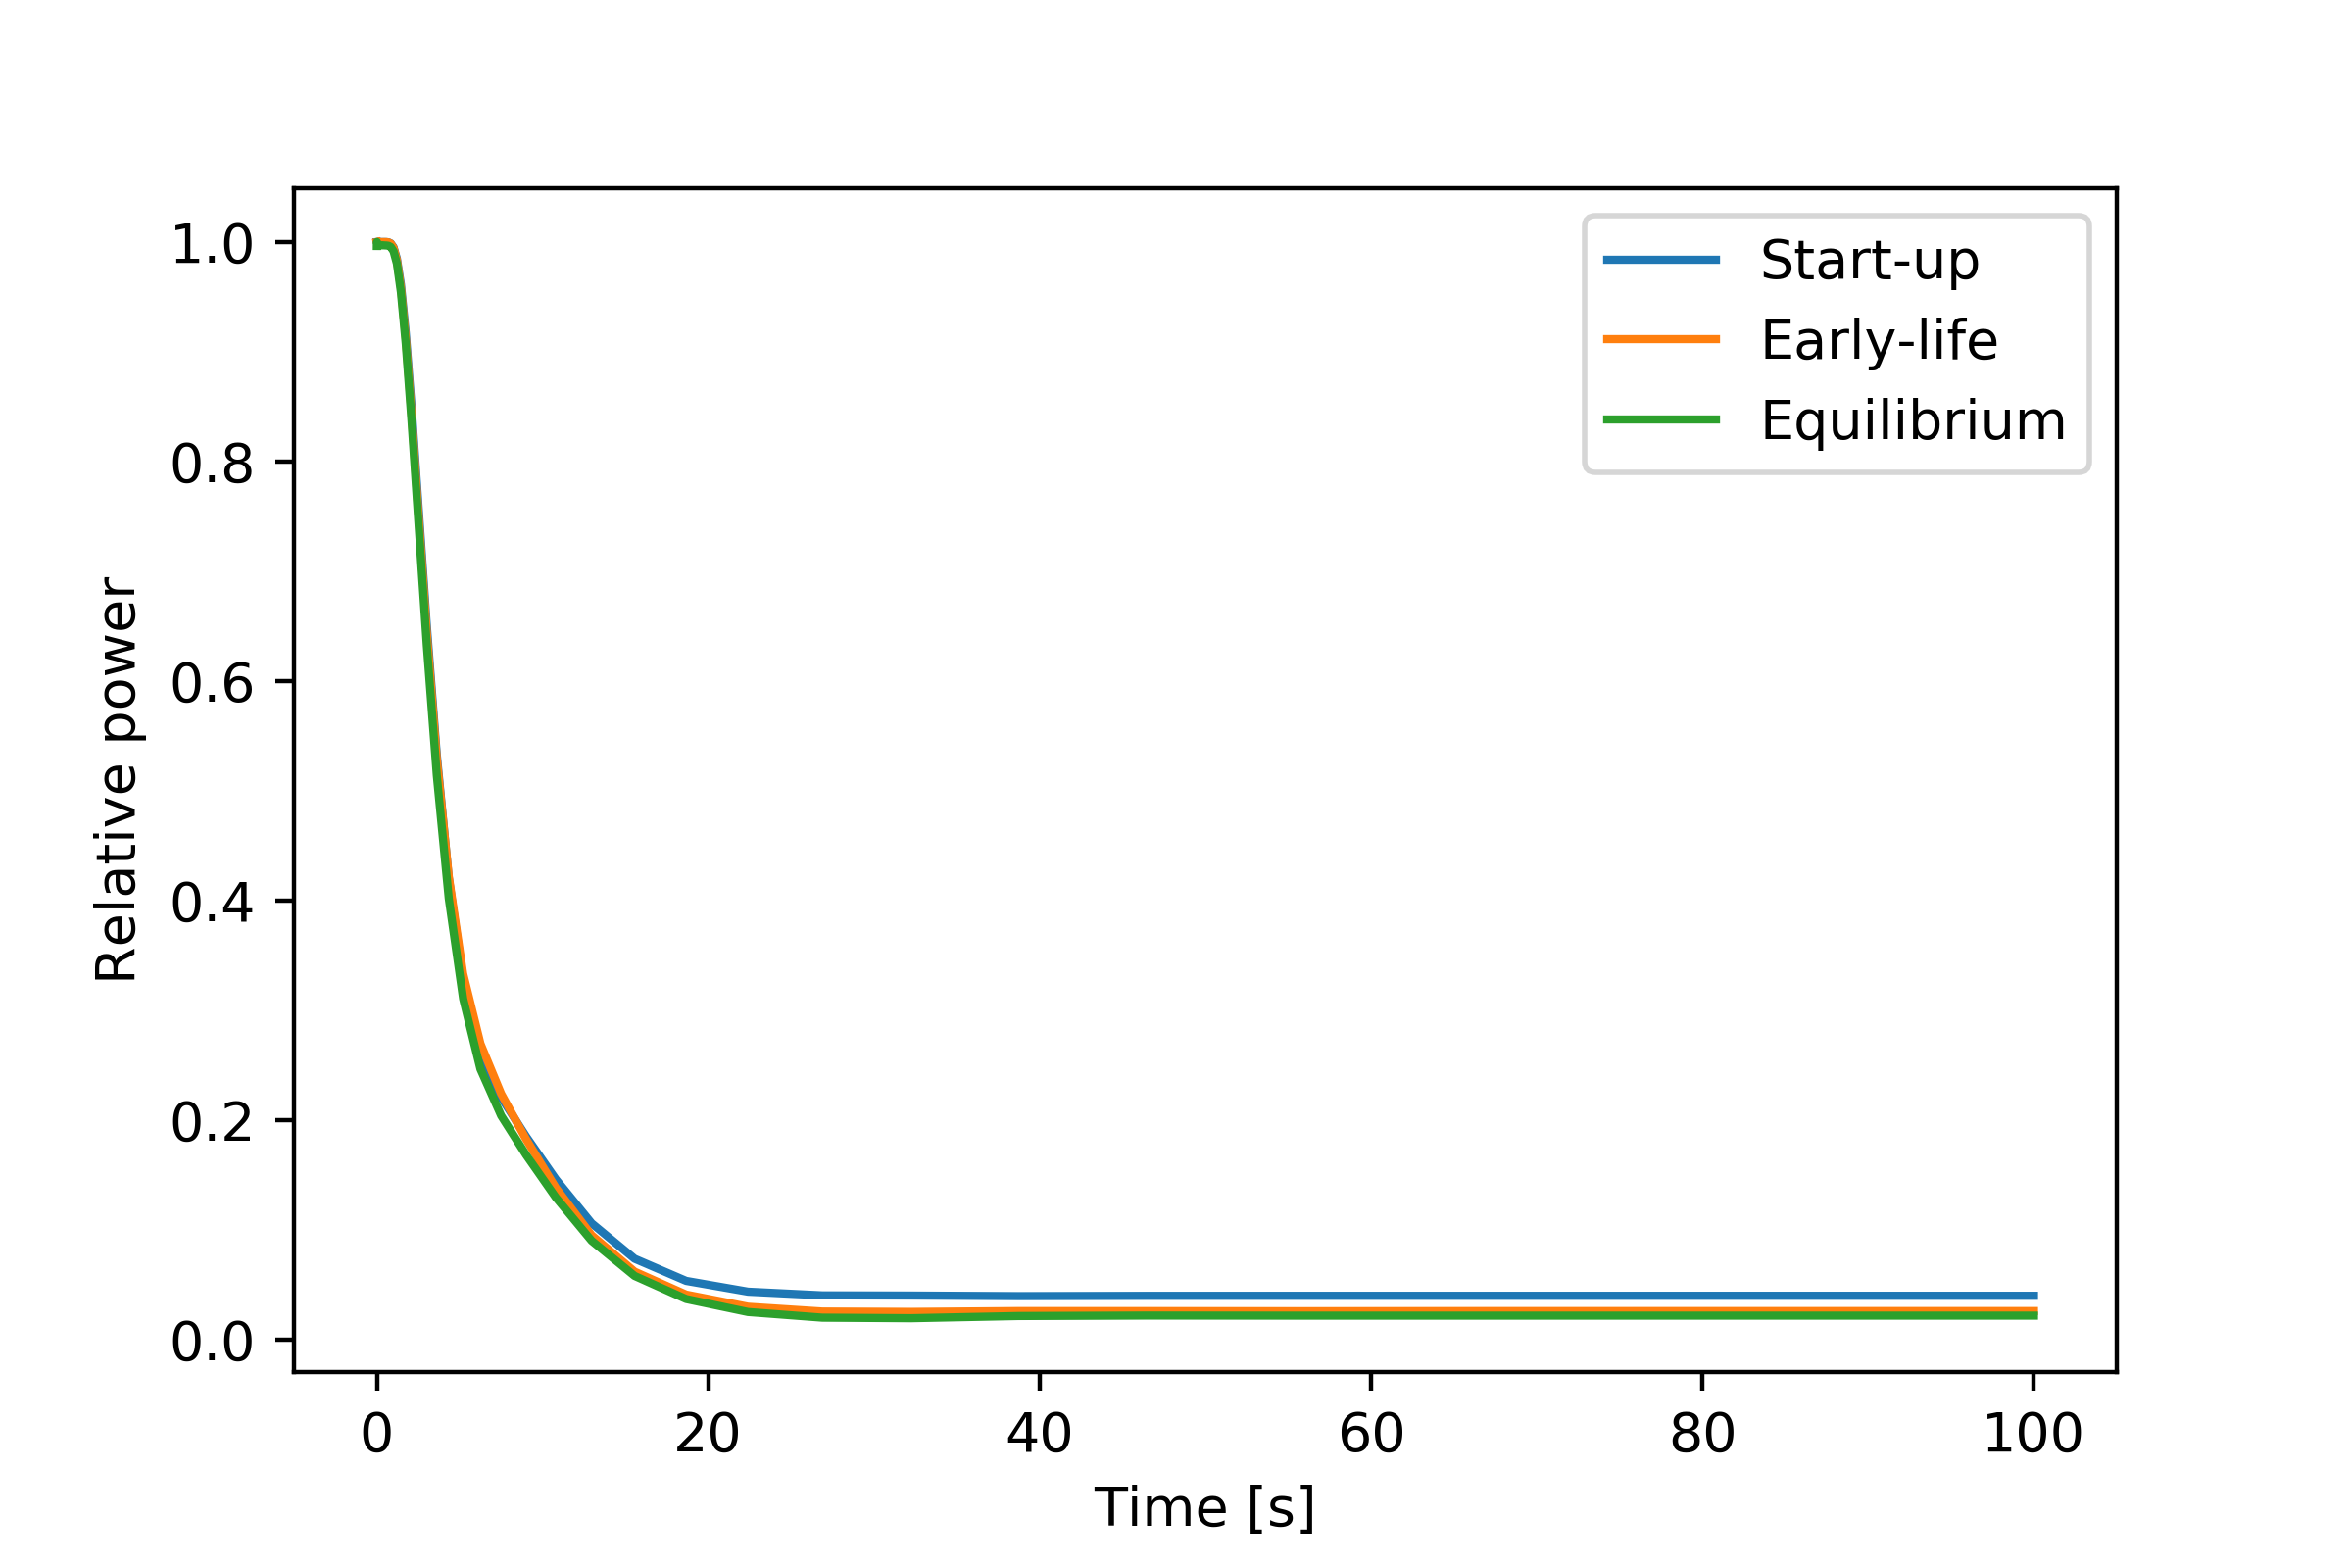
\includegraphics[height=2.8cm]{./images/loscaheat}
    			\caption{\scriptsize Clockwise from top left: MSFR 2D
    			axisymmetric mesh, steady state fuel temperature distribution,
    			relative power during a loss of heat sink scenario.}
			\end{figure}
			\vspace{.1cm}
			\column[t]{.5\textwidth}
			\begin{figure}
				\centering
				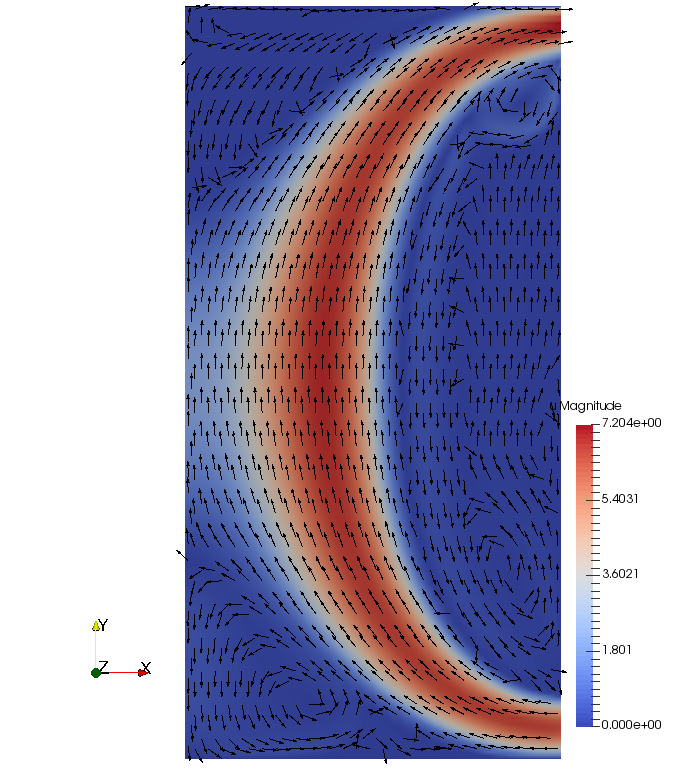
\includegraphics[width=.9\textwidth]{./images/ins-flow}
				\caption{\footnotesize Velocity distribution produced from the
				incompressible Navier-Stokes equations}
			\end{figure}
		\end{columns}
\end{frame}
\begin{frame}
	\frametitle{Ansh - Energy Analysis for Decarbonization in Japan}
	% a comment
  \begin{figure}[htbp!]
    \begin{center}
      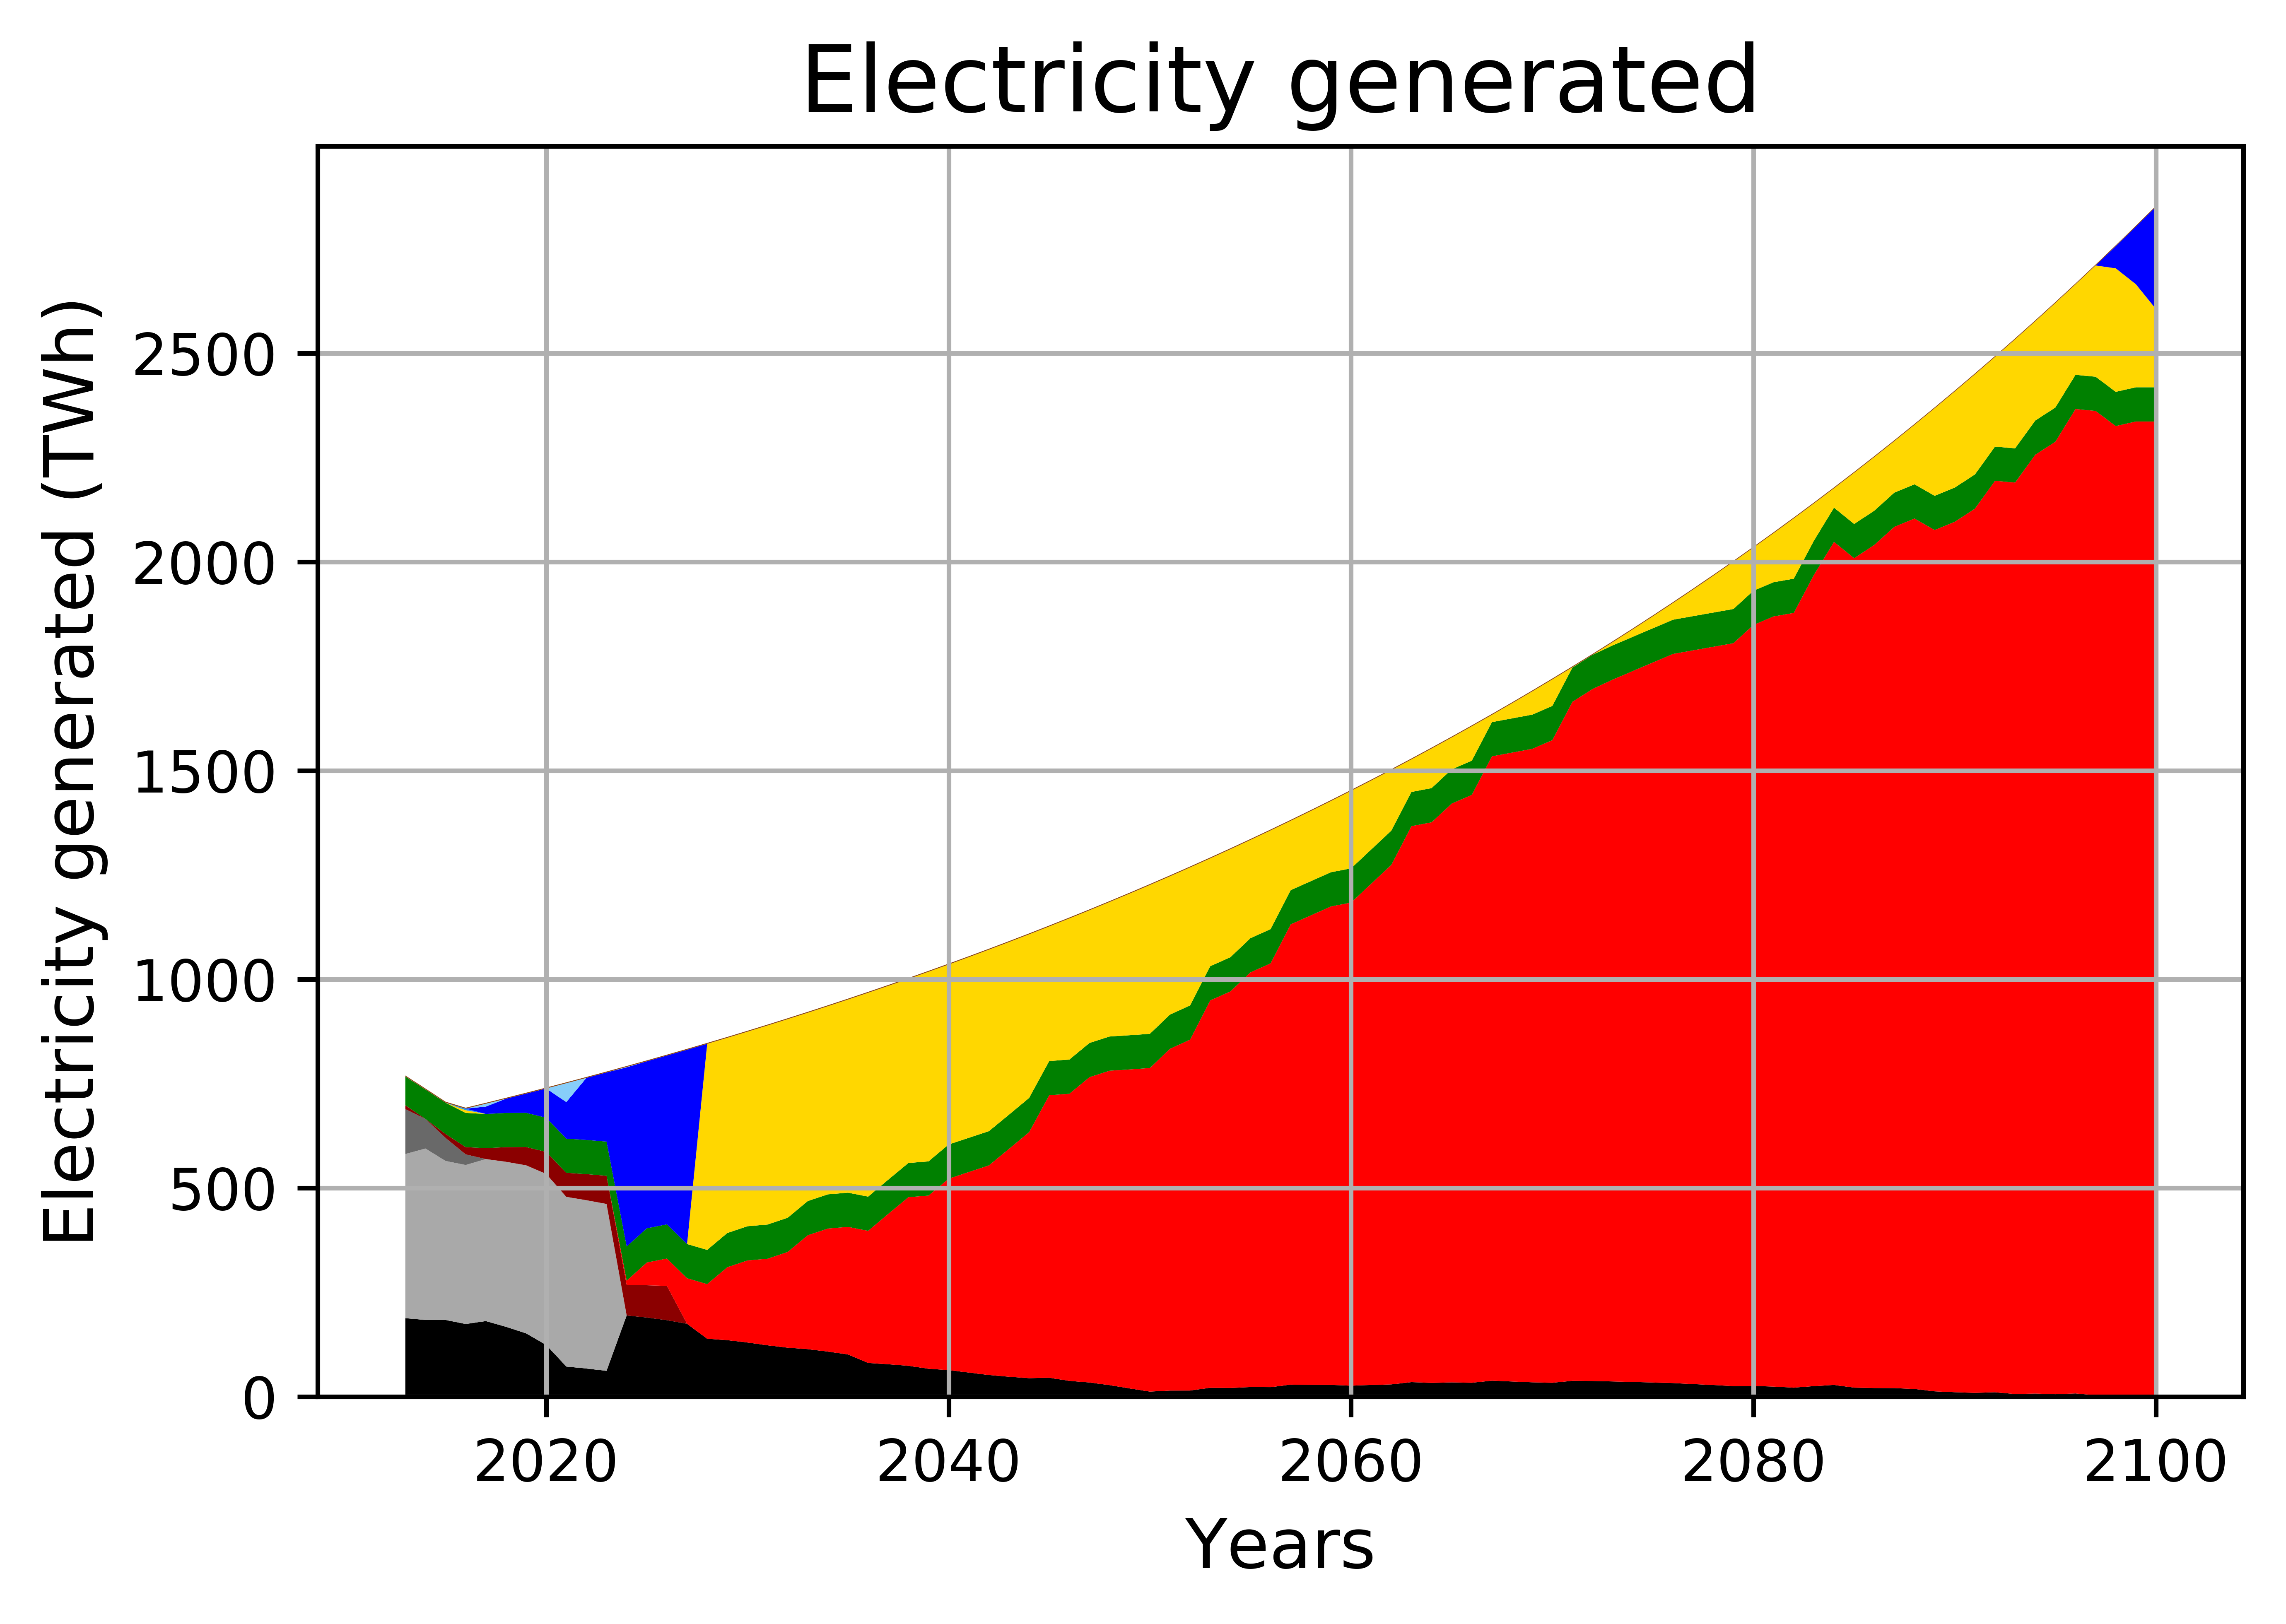
\includegraphics[scale=0.5]{./images/conv_nuc_elc}
    \end{center}
          \caption{Electricity generation in Japan without constraints on nuclear energy. Scenario simulated using TIMES.}
    \label{s1e}
  \end{figure}

\end{frame}

\begin{frame}
	\frametitle{Ansh - Recirculation zones in MSRE}
	% a comment
  \begin{figure}[htbp!]
    \begin{center}
      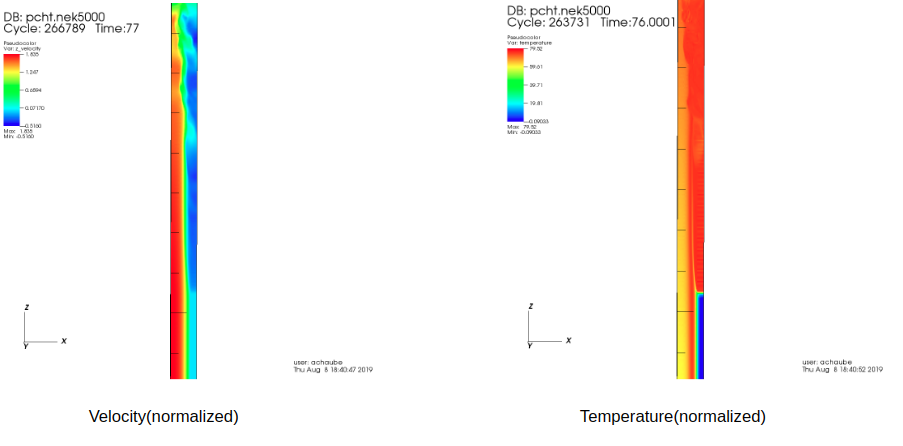
\includegraphics[scale=0.35]{./images/msre-flat}
    \end{center}
          \caption{LES simulation of MSRE channel without pyramid stringer using Nek5000.}
    \label{s1e}
  \end{figure}

\end{frame}

\begin{frame}
\frametitle{Transatomic Power (TAP) concept high-fidelity Serpent model}
	  \begin{textblock*}{12.25cm}(0.25cm,1.8cm) % {block width} (coords)
\begin{figure}[htp!] % replace 't' with 'b' to 
	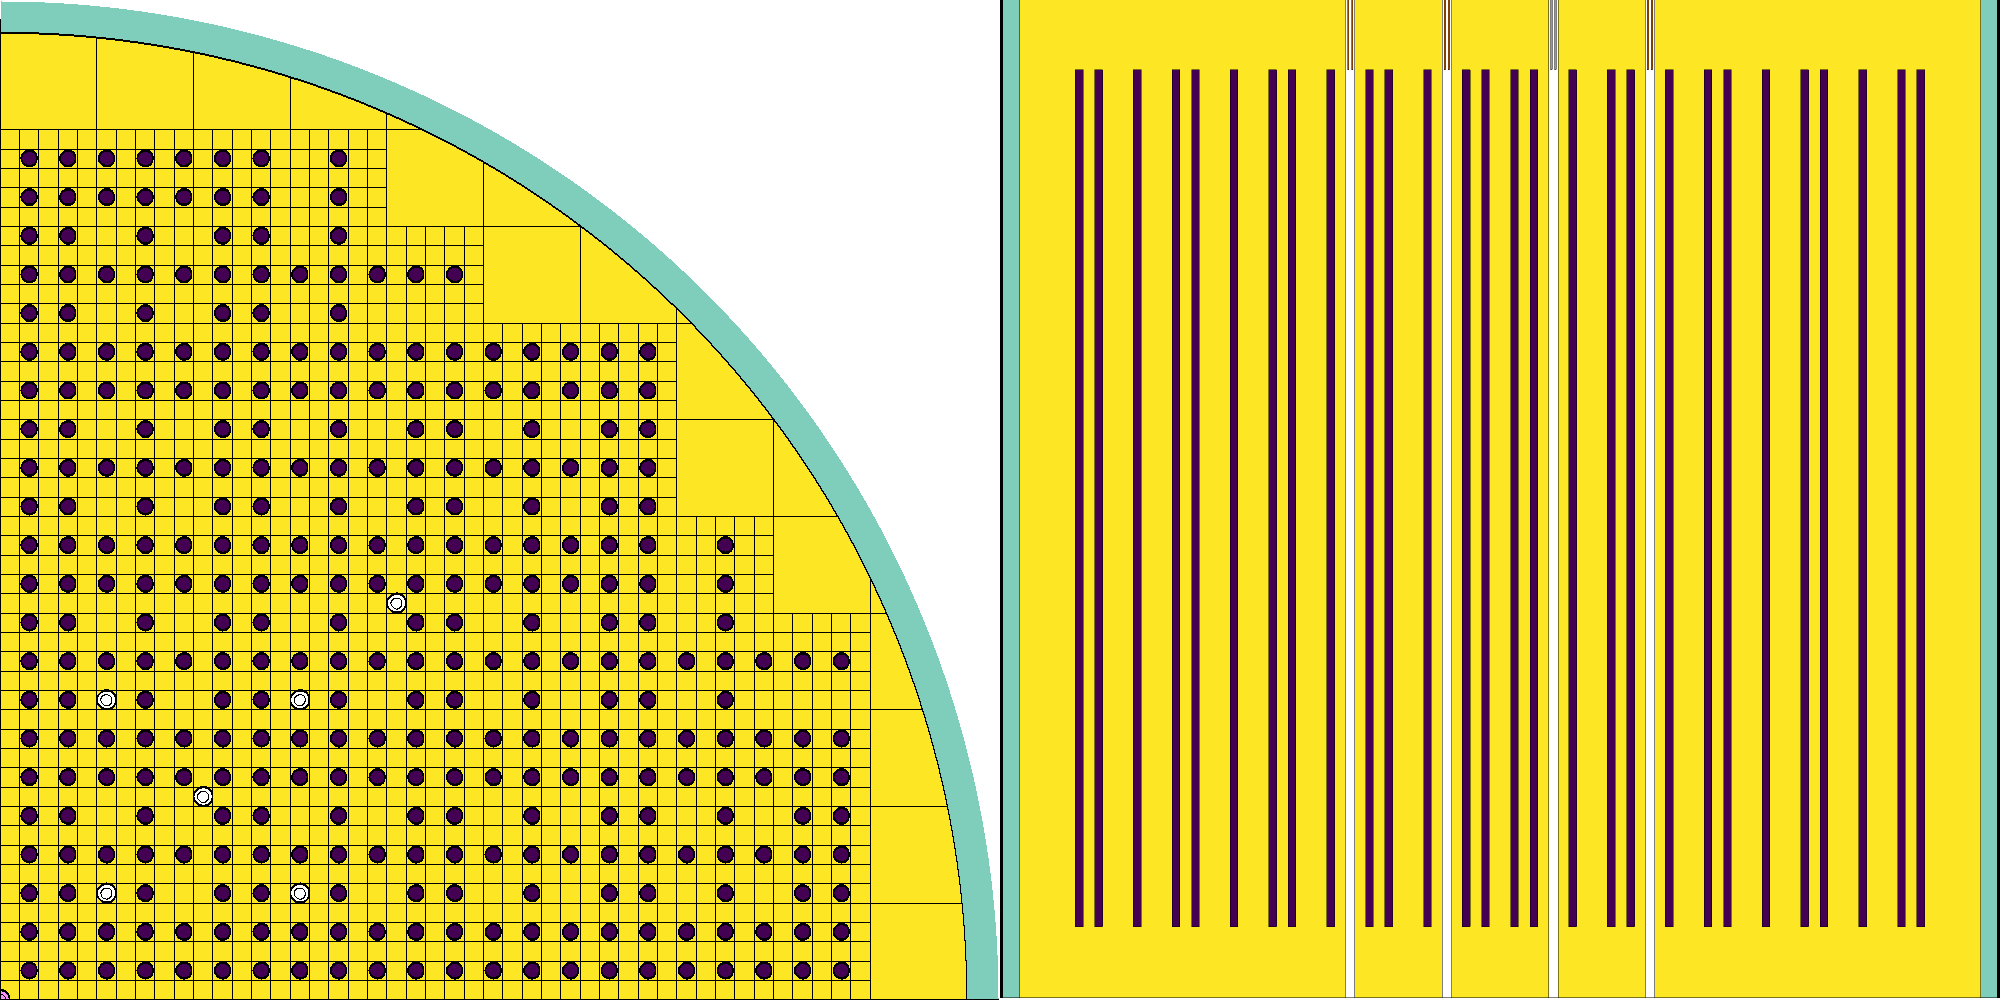
\includegraphics[width=\textwidth]{./images/tap_model.png}
	\caption{An $XY$ (left) and $XZ$ (right) section of the TAP model. 
	The violet color represents zirconium hydride, and the yellow represents 
	fuel salt (reproduced from Rykhlevskii \& Huff, Milestone 2.1 Report, 
	2019).}
\end{figure}
	  \end{textblock*}
\end{frame}


\begin{frame}
\frametitle{Depletion simulation results for TAP with various feeds}       
\begin{textblock*}{12.6cm}(0.1cm,2.2cm) % {block width} (coords)
	\begin{figure}[htp!] % replace 't' with 'b' to 
		\begin{minipage}[b]{0.48\textwidth}
			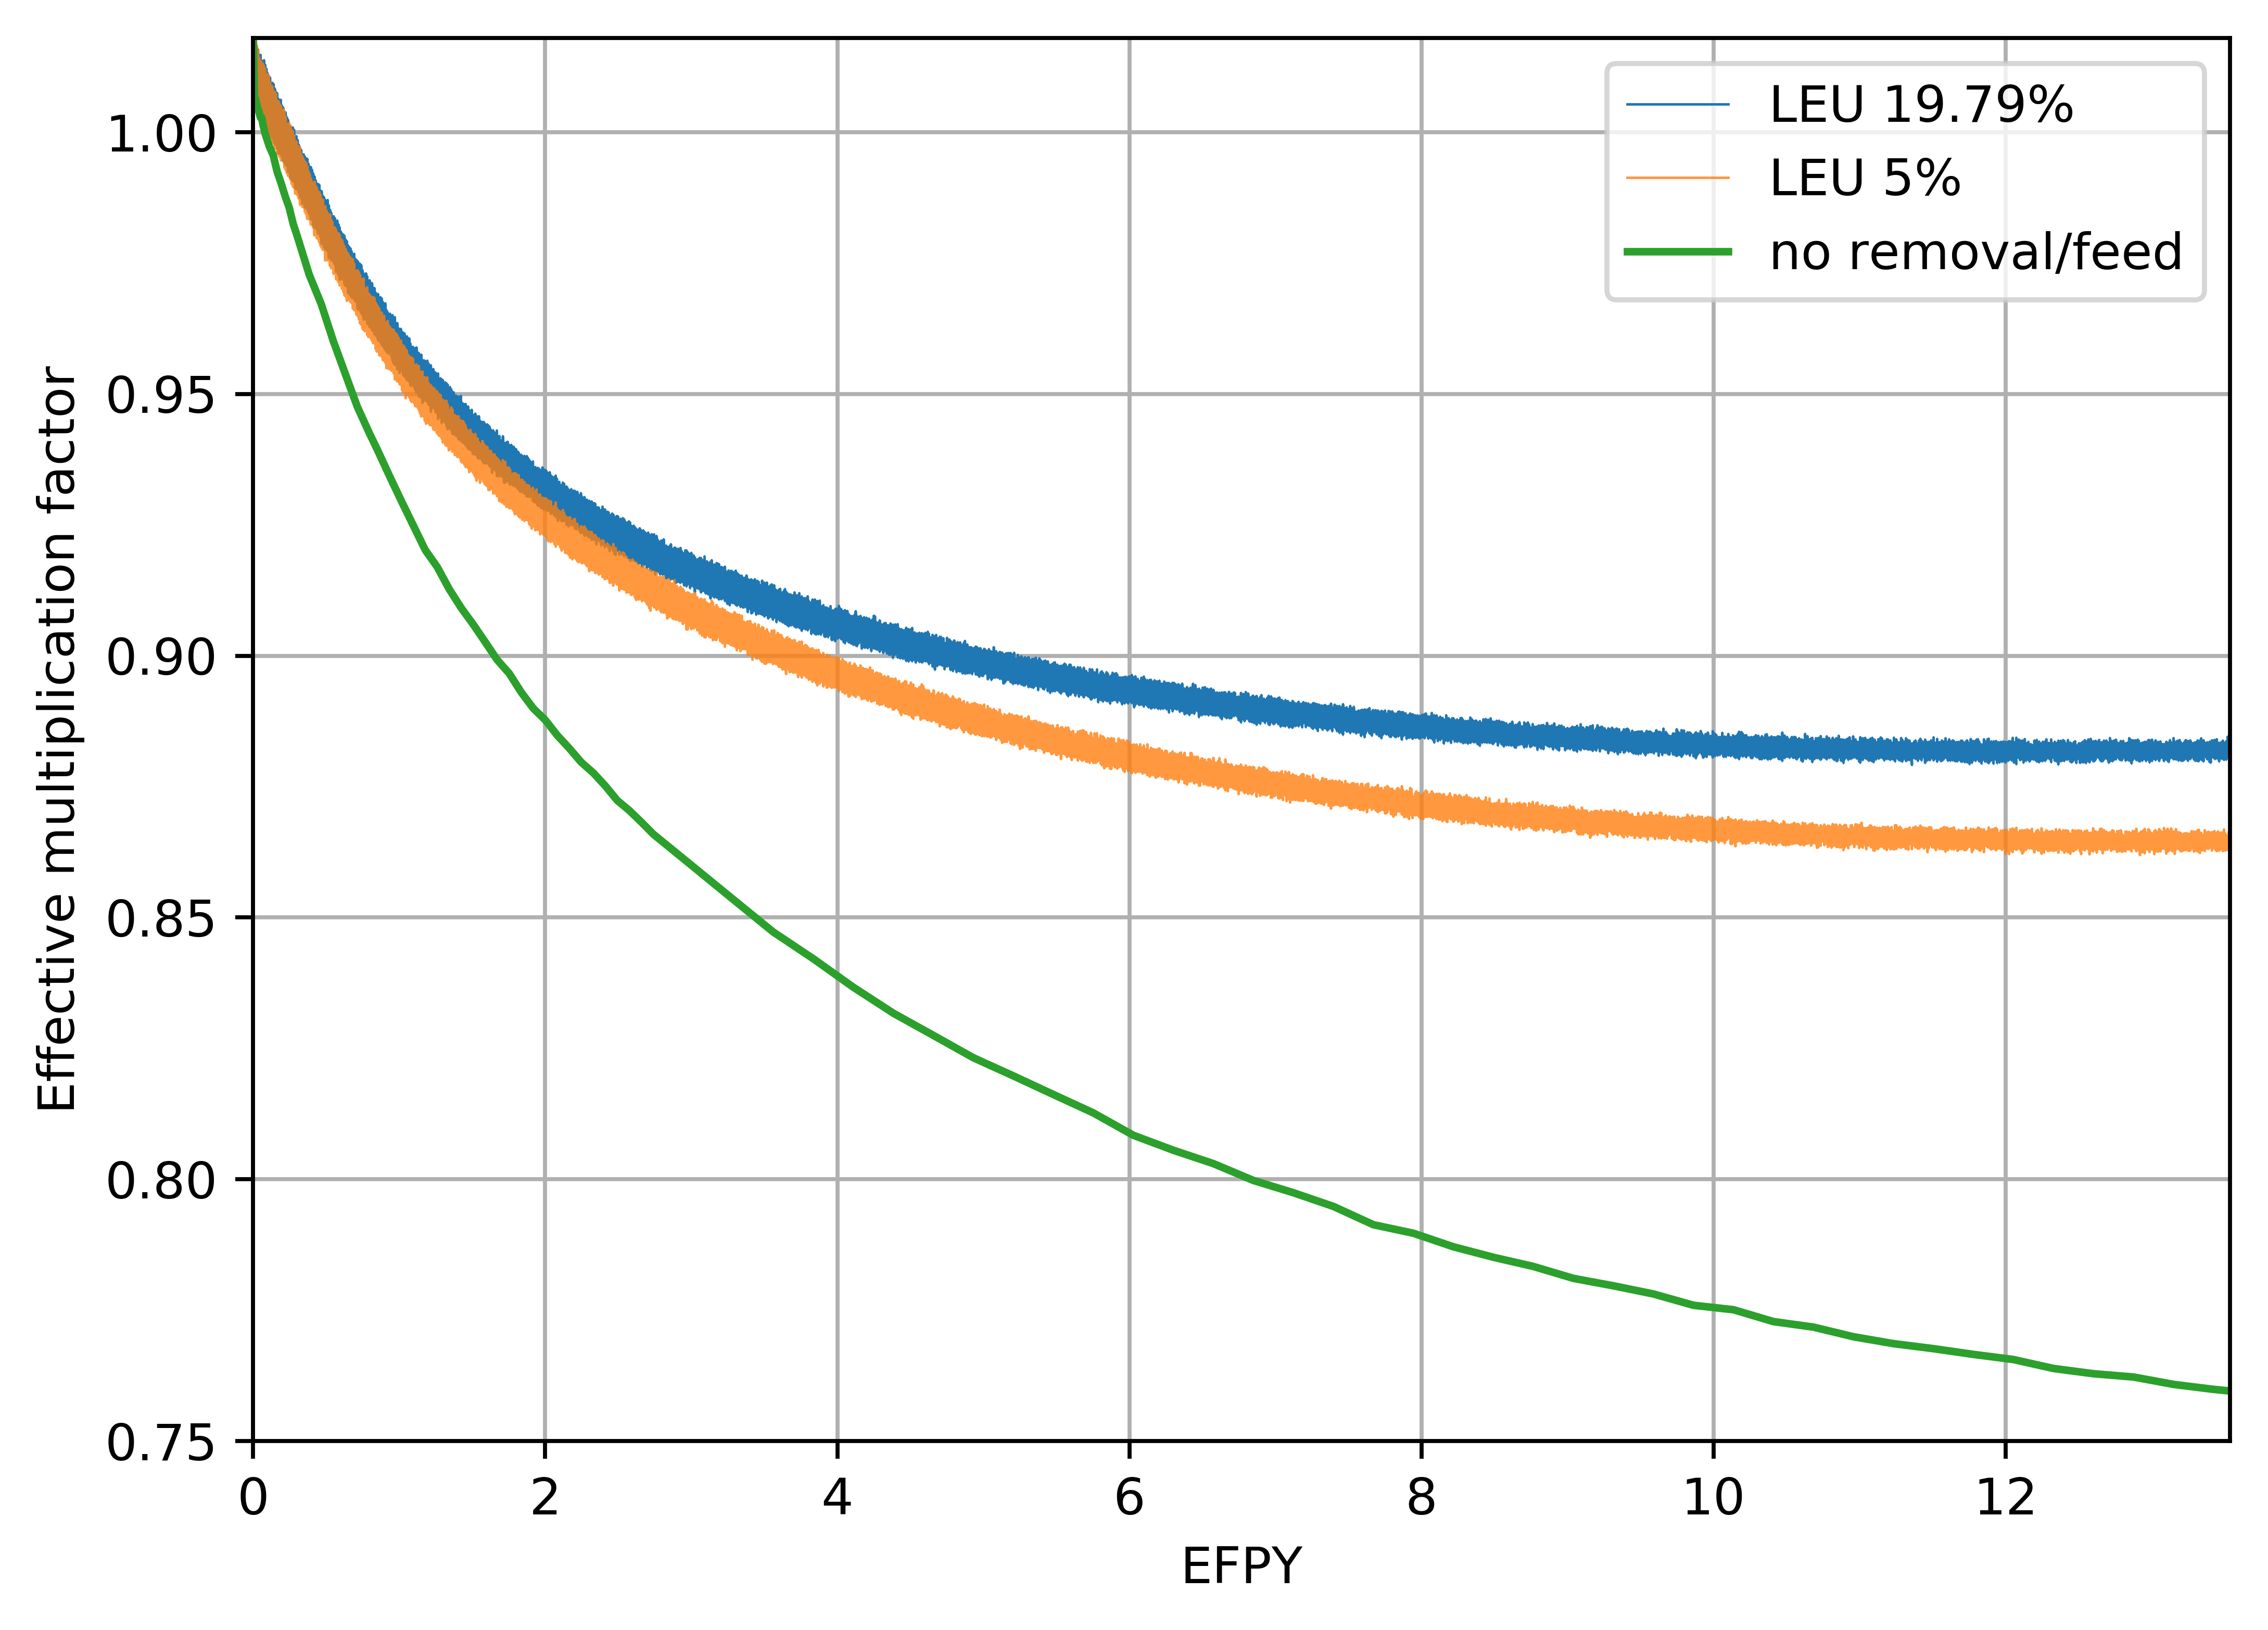
\includegraphics[width=\linewidth]{./images/keff_3.png}
		\end{minipage}
			\hspace{-2mm}
		\begin{minipage}[b]{0.48\textwidth}
			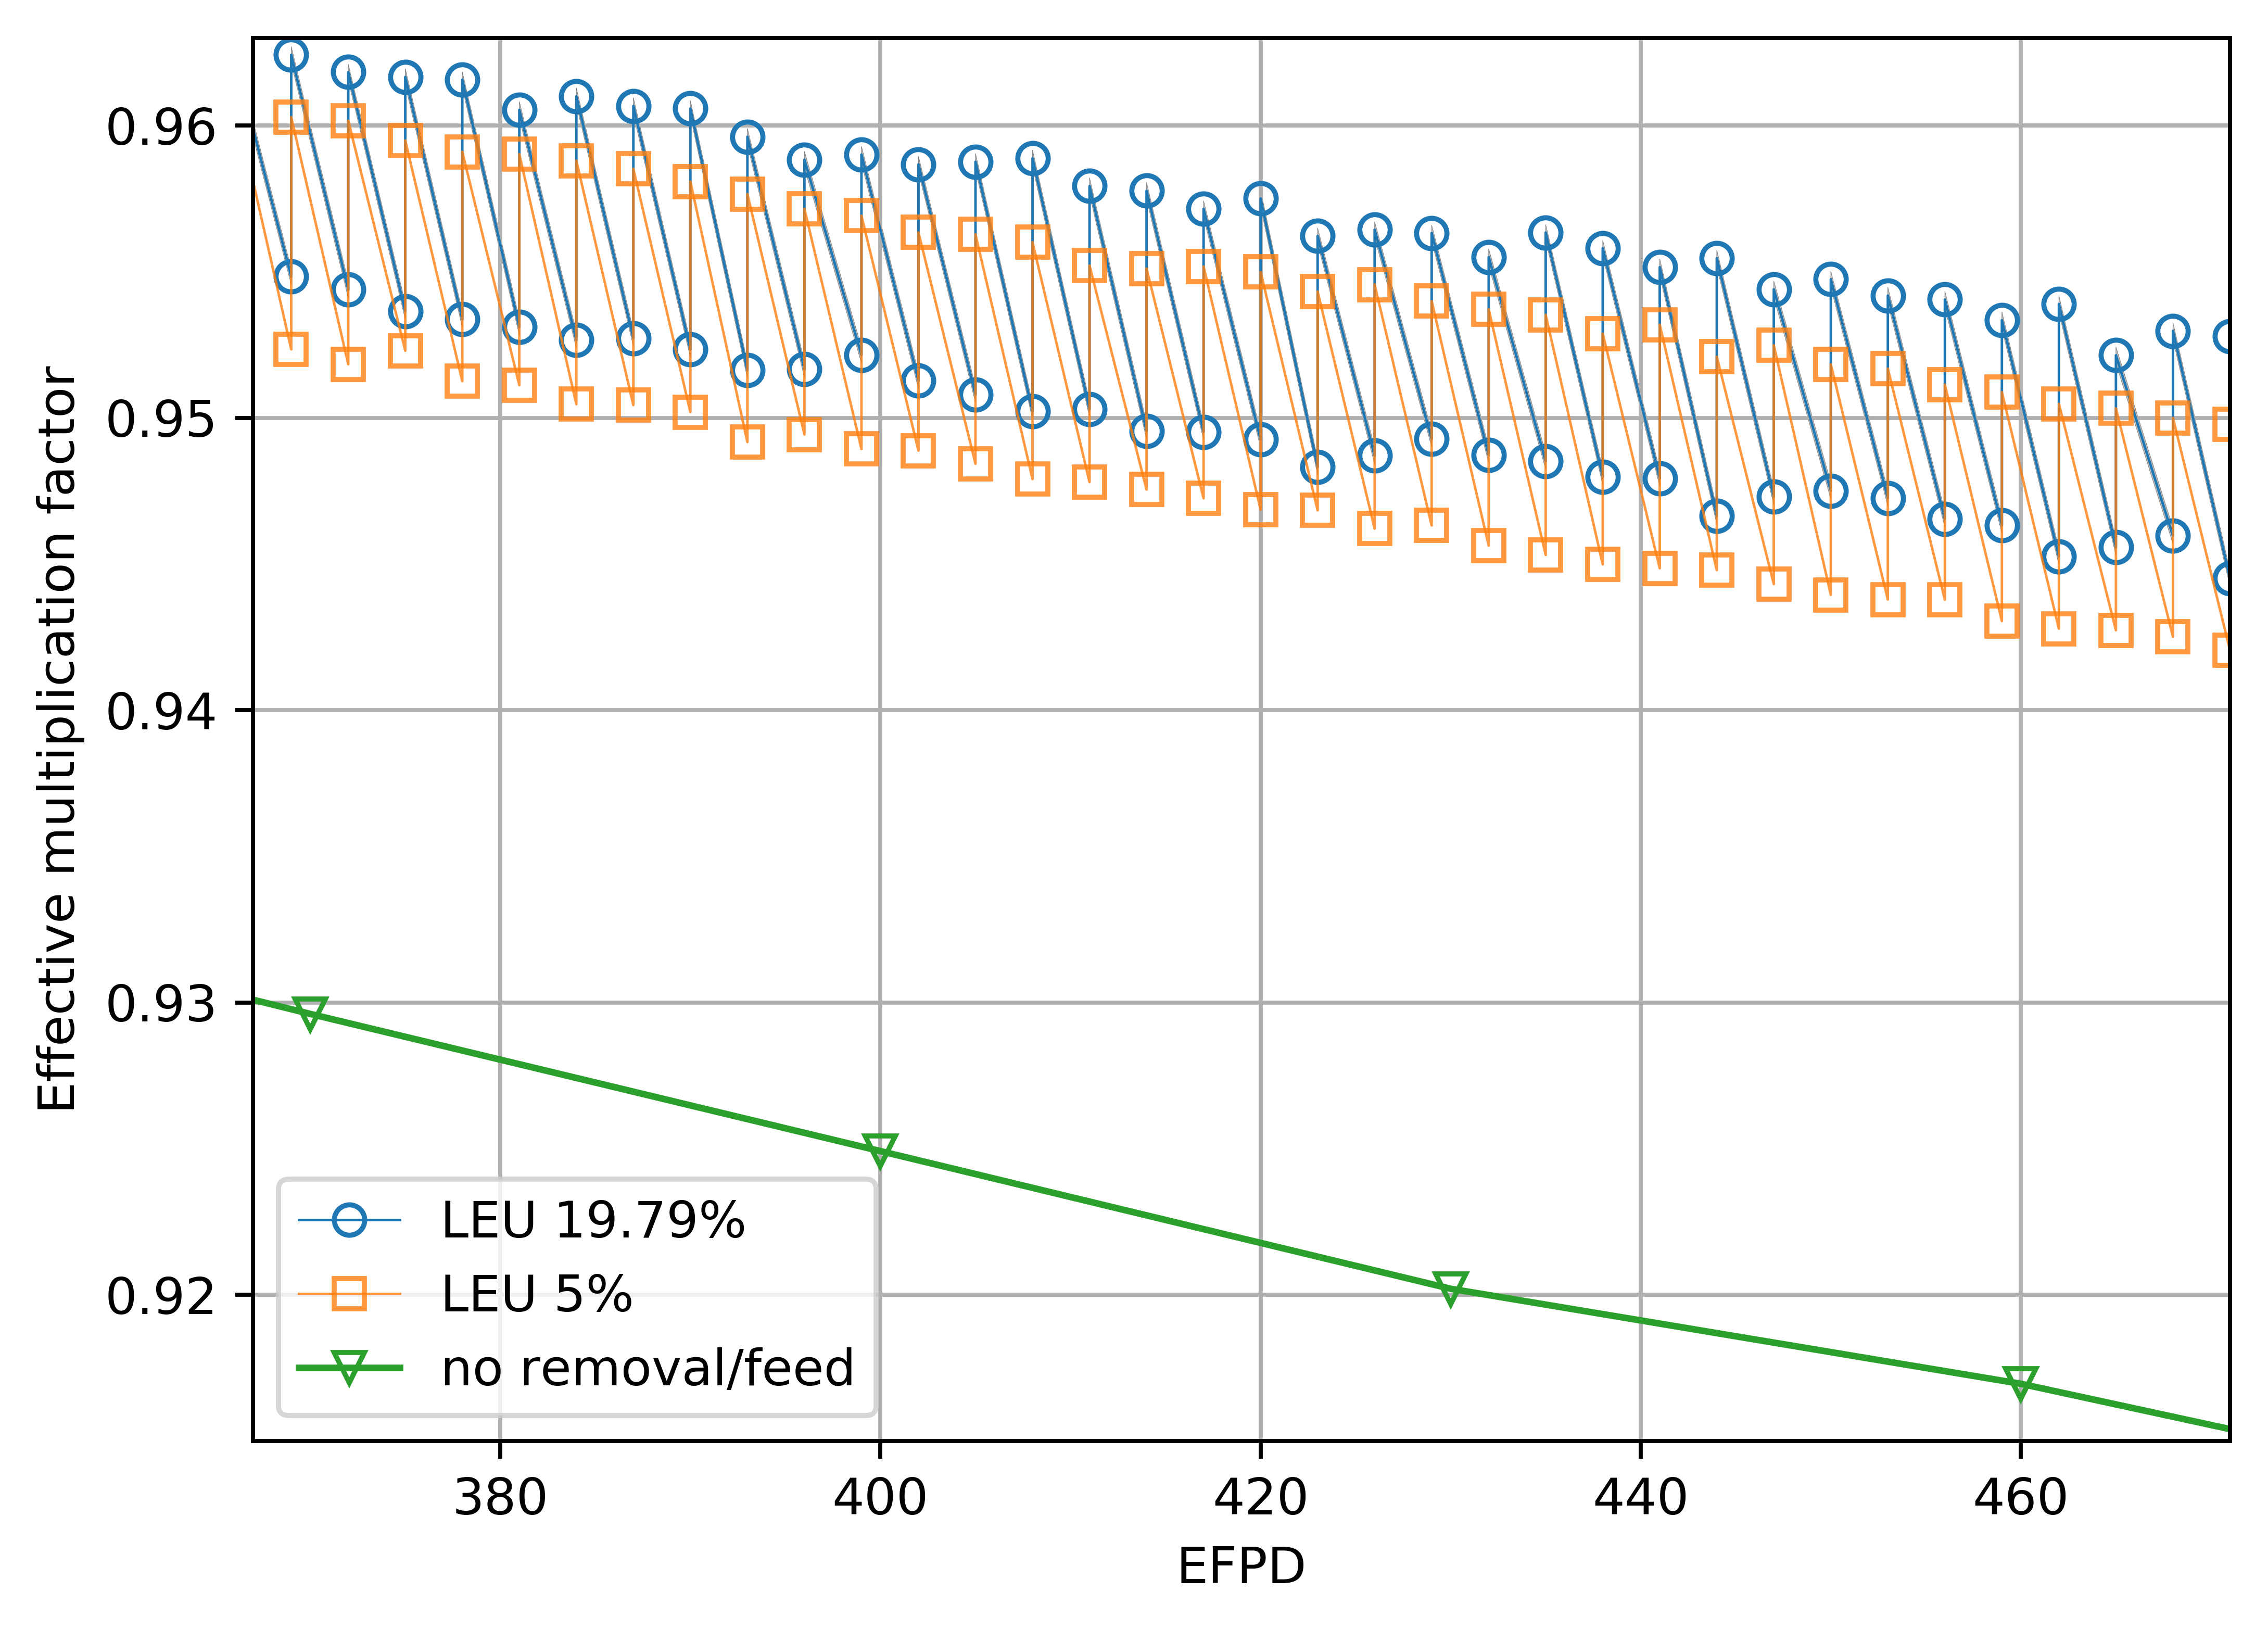
\includegraphics[width=\linewidth]{./images/keff_zoomed_2.png}
		\end{minipage}
		\caption{Effective multiplication factor dynamics for full-core
		TAP model for different fueling scenarios over a 13-year reactor 
		operation (left) and for the time interval from 367 to 471 days after 
		startup (right). Confidence interval $\pm\sigma=28pcm$ is shaded.}
	\end{figure}
\end{textblock*}
\end{frame}


\begin{frame}
\frametitle{Fuel salt composition evolution during the TAP operation}
\begin{textblock*}{12.25cm}(0.25cm,2cm) % {block width} (coords)
	\begin{figure}[htp!] % replace 't' with 'b' to 
		\centering
				\vspace{-3mm}
		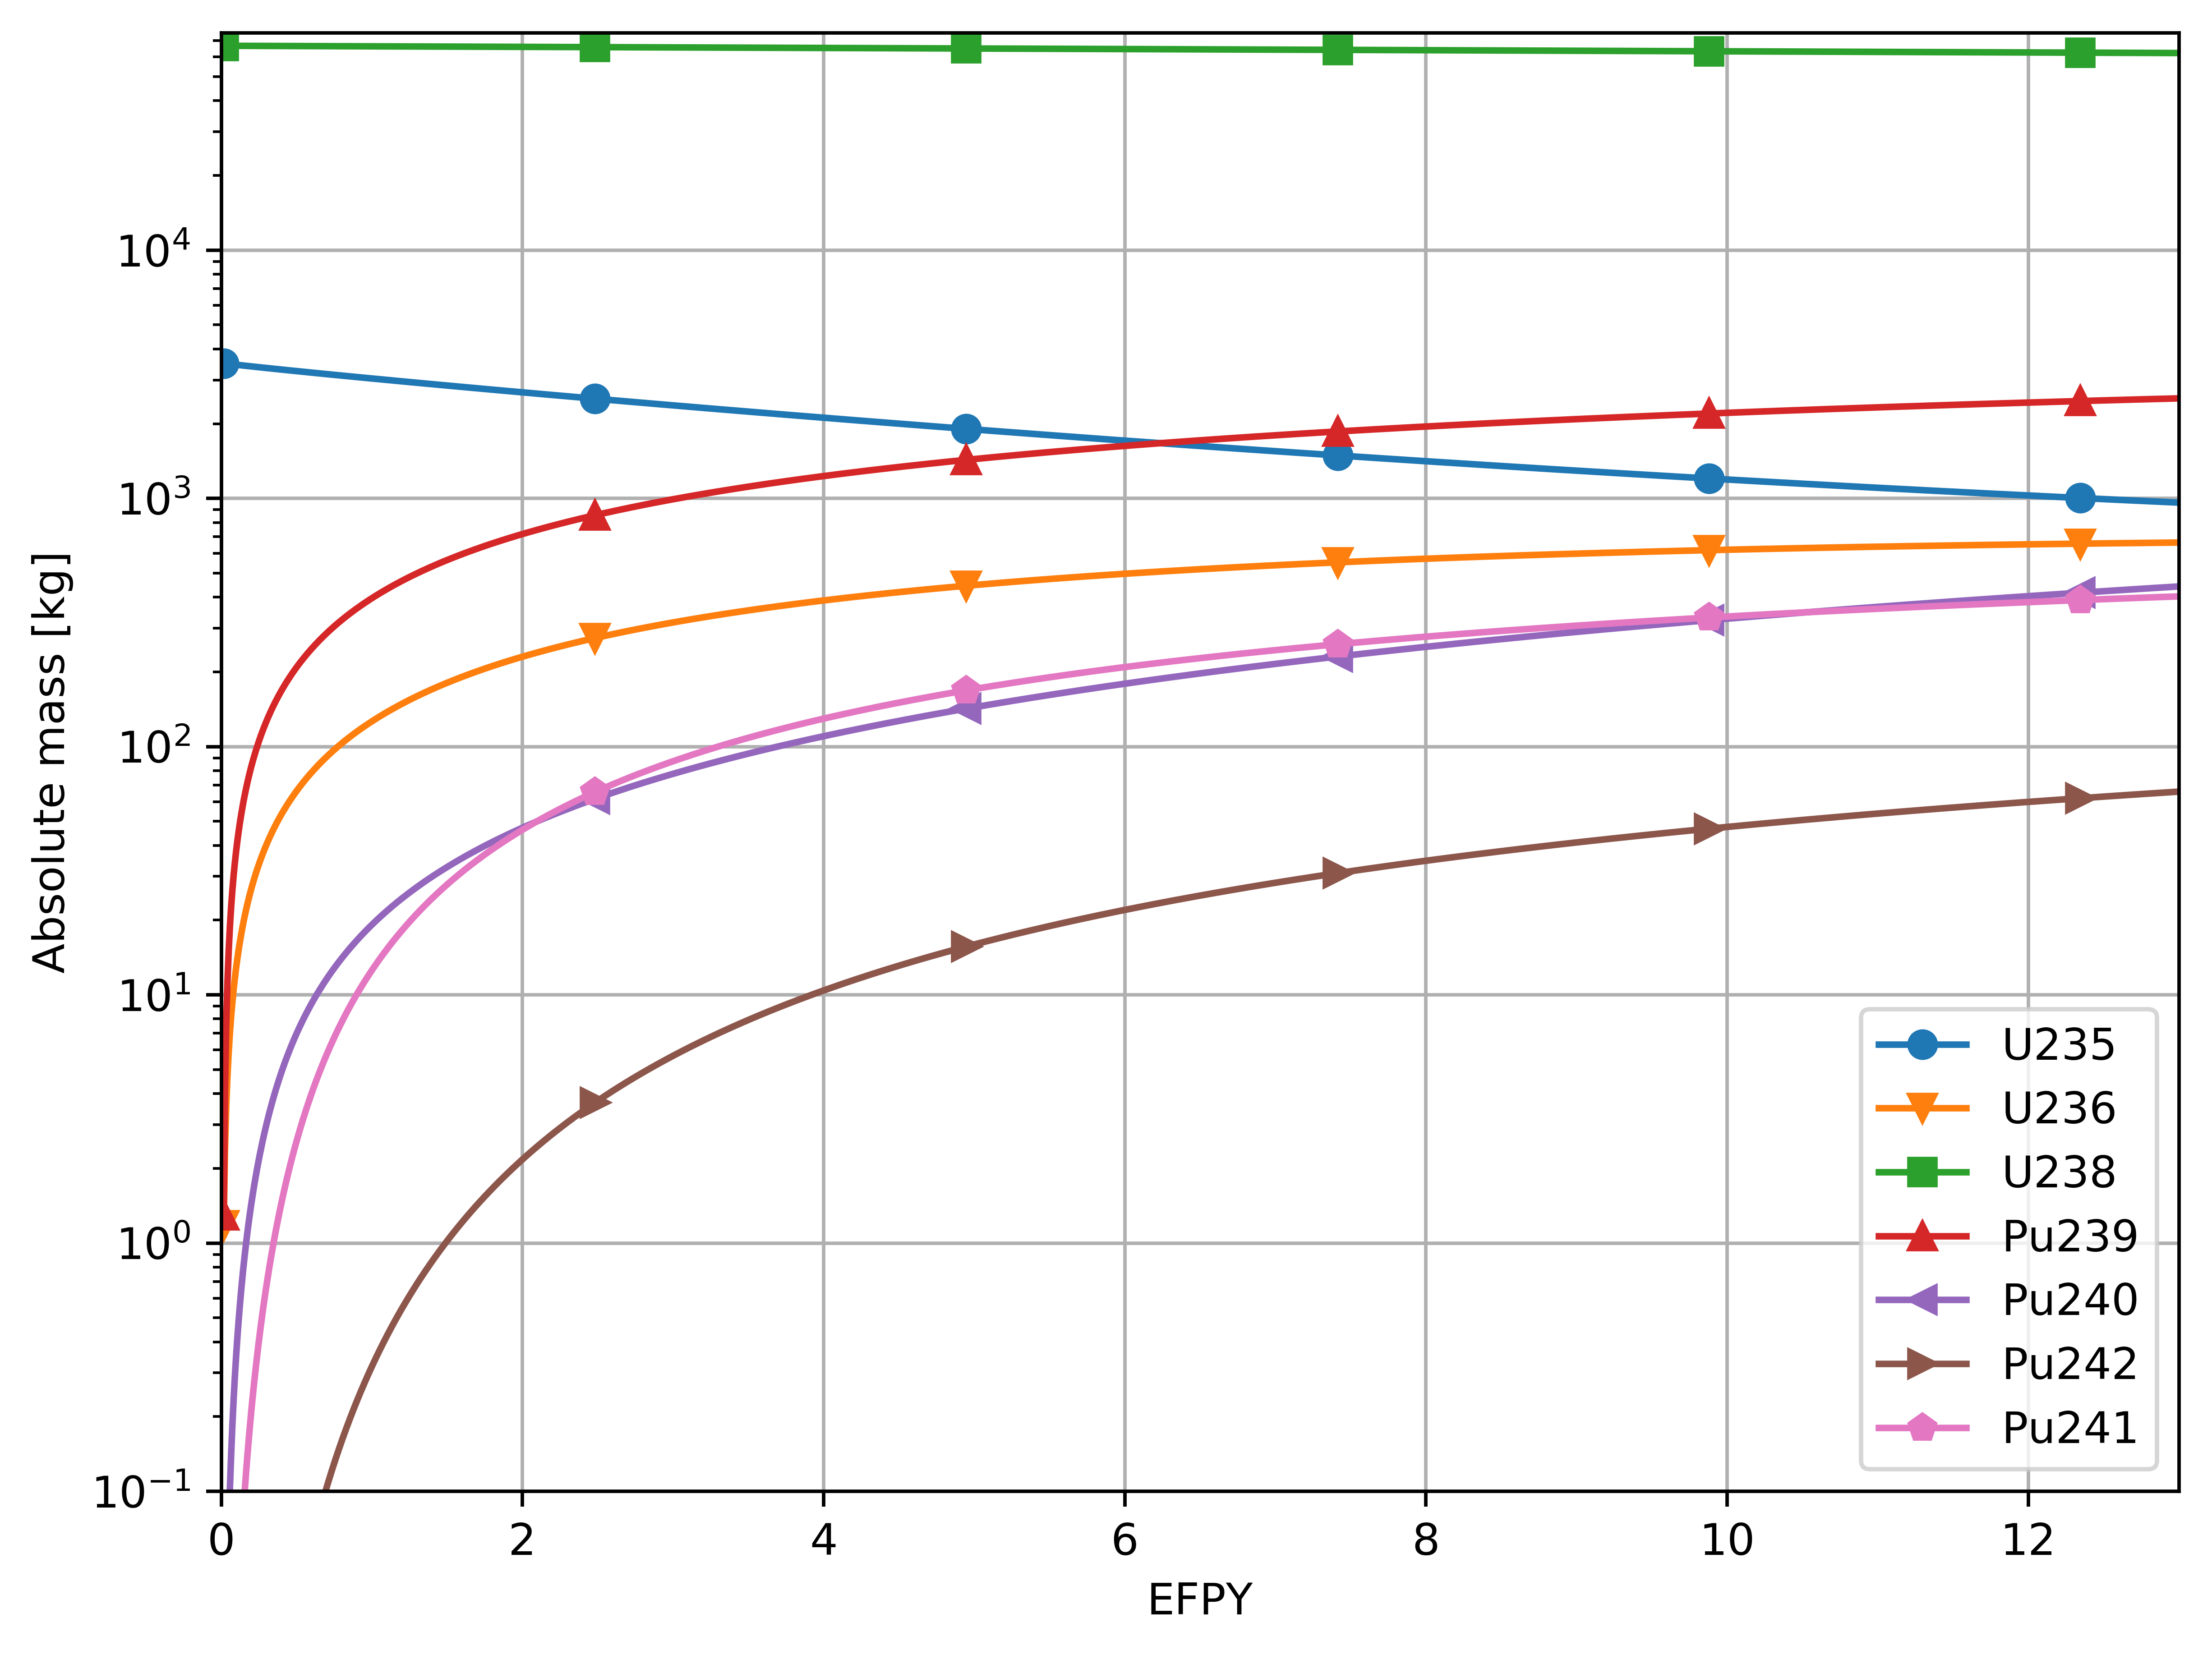
\includegraphics[width=0.72\textwidth]{../images/u_pu_mass.png}
		\caption{Mass of major nuclides during 13 years of reactor operation 
		with 19.79\% low-enriched uranium feed.}
	\end{figure}
\end{textblock*}
\end{frame}
\input{richter}
\begin{frame}
	\frametitle{Roberto Fairhurst: Compressibility in Moltres}
		\begin{columns}
		\column[t]{6cm}

		Compressibility in liquids:
		
            \begin{align}
			\rho (\vec{v}.\nabla)\vec{v} + \nabla p - \rho g \check{j} - \mu \nabla^{2}\vec{v} = 0 \\
			\vec{v}.\nabla\rho+\rho\nabla.\vec{v}=0 \\
			\rho c_{v} (\vec{v}.\nabla)T - \nabla .(k\nabla T) + p (\nabla . \vec{v})= 0 \\
			\rho = \rho_{0} + \frac{\rho_{0}}{K}(p-p_{0}) + \rho_{0}\beta(T-T_{0})
            \end{align}

			\begin{itemize}
				\item Density dependency on pressure and temperature for liquids.
				\item Next, implement it for gasses $p=\rho RT$
			\end{itemize}

		\column[t]{5cm}
		\begin{figure}[htbp!]
			\begin{center}
				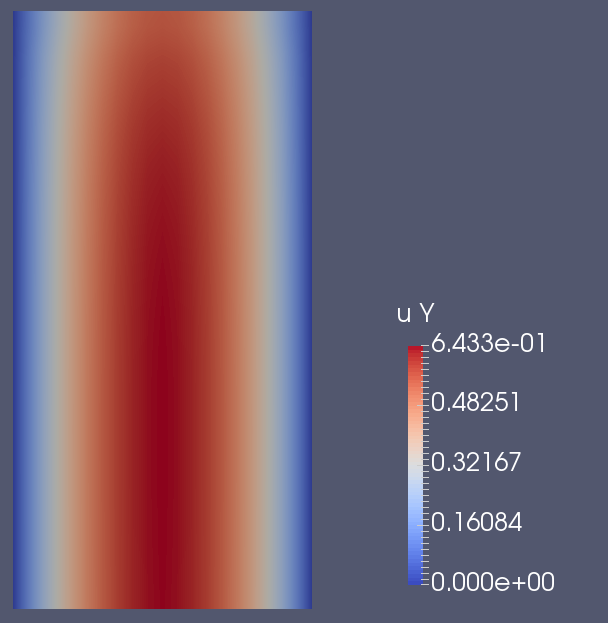
\includegraphics[height=2cm]{./images/liquid_compres.png}
			\end{center}
			\caption{Vertical velocity.}
			\label{fig:velocity}
		\end{figure}

		\begin{figure}[htbp!]
			\begin{center}
				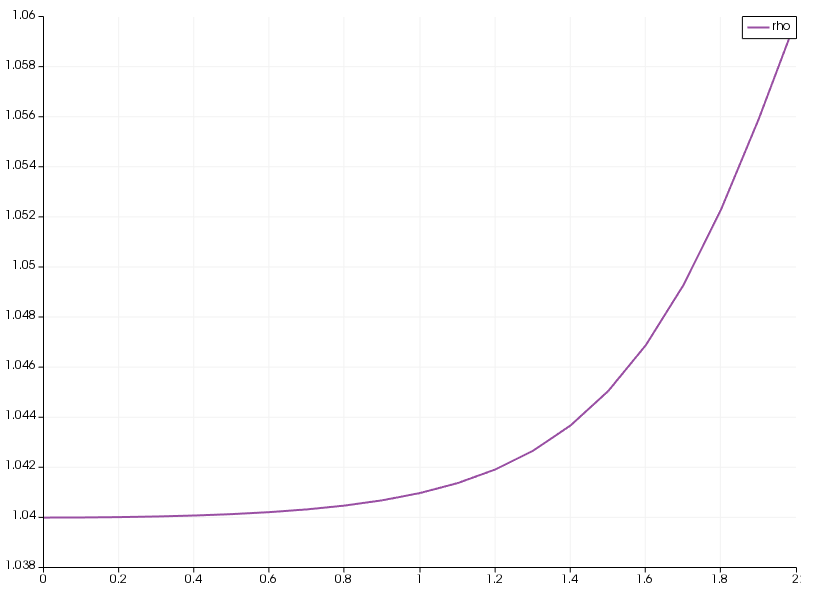
\includegraphics[height=2cm]{./images/rho.png}
			\end{center}
			\caption{Density distribution.}
			\label{fig:density}
		\end{figure}

		\end{columns}
\end{frame}
\section{Fuel Cycles}
\begin{frame}
  \frametitle{Diversion Detection with Cyclus}
  	\textbf{Motivation}
        \begin{itemize}
                \item Safeguard by design
                \item Model diversion inside facilities
                \item transition from LWR to SFR
        \end{itemize}
    \textbf{Goals}
    	\begin{itemize}
    		\item Detect diversion using signatures and observables.
    		\item Optimum detector and inspection locations in pyroprocessing
    		\item Characterize detection sensitivities and false positive rates
    	\end{itemize}
  \begin{figure}
    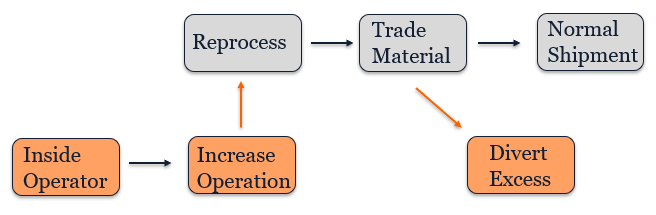
\includegraphics[width=0.7\linewidth]{./images/westphal-diversion}
    \caption{Operator vs nefarious diversion.}
    \label{fig:diversion}
  \end{figure}
\end{frame}

\begin{frame}
	\frametitle{PyRe Archetype}
	\begin{columns}
		\column[t]{6cm}
		\begin{itemize}
			\item Facility containing multiple sub-processes:
			\begin{itemize}
				\item Separately handled.
				\item Independent transactions, possibility of diversion.
			\end{itemize}
			\item Operation setting impact efficiency.
			\item Generic facility:
			\begin{itemize}
				\item Multiple types of pyro plants.
				\item LWR vs SFR.
			\end{itemize}
		\end{itemize}
		\begin{block}{Diversion Detection}
			Material transactions are no longer a reliable method. Instead we use
			signatures and observables:
			\begin{itemize}
				\item Temperature, power draw, etc.
			\end{itemize}
			A Cumulative Sum change algorithm is used to detect any significant changes.
		\end{block}
		\column[t]{5cm}
		\begin{figure}
			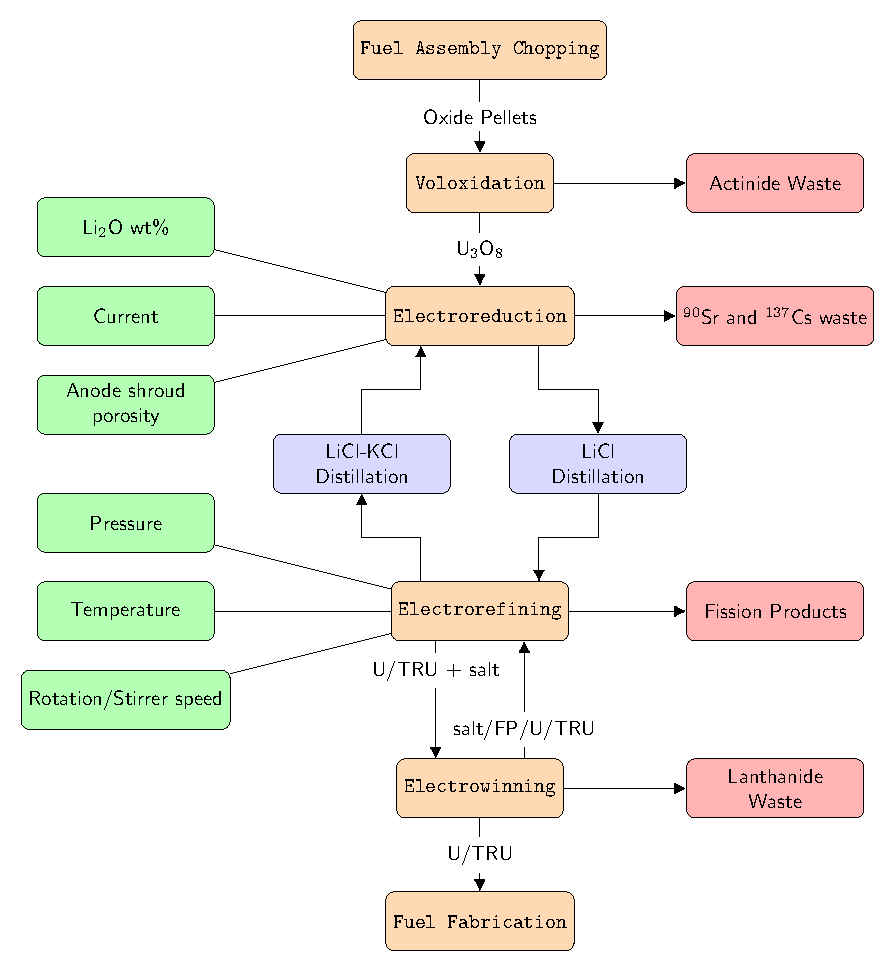
\includegraphics[width=\linewidth]{./images/westphal-pyre.pdf}
			\caption{PyRe flow diagram for LWR waste configuration.}
			\label{fig:pyre}
		\end{figure}
	\end{columns}
\end{frame}
\begin{frame}
    \frametitle{Sensitivity Analysis with Fuel Cycle Codes}
    \textbf{Motivation for conducting sensitivity analysis}
    \\

    A transition scenario is simulated to predict the 
    future, however when implemented in the real world, 
    it will deviate from the optimal scenario. 
    Therefore, sensitivity analysis studies is necessary to 
    determine how variation in different parameters will impact 
    the progression and final state of the transition scenario. 
    \\

    \textbf{Method}

    Couple fuel cycle codes, \textsc{Cyclus}/DYMOND, 
    with Dakota \cite{eldred_dakota_2010} (sensitivity analysis, 
    optimization, and uncertainty quantification framework).  

    \begin{figure}[]
        \centering
        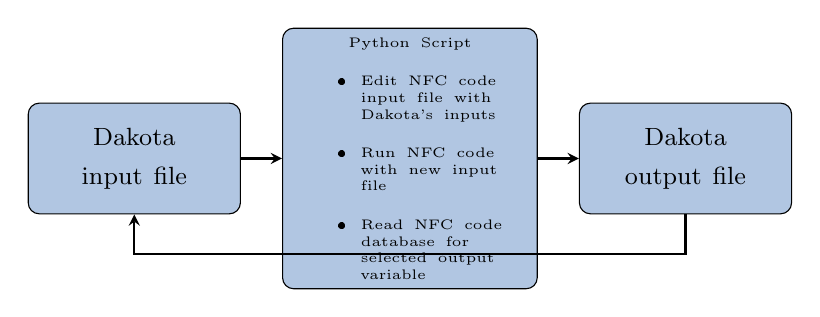
\begin{tikzpicture}[node distance=2.5cm]
            \tikzstyle{every node}=[font=\large]
            \node (one) [sbblock]{\small Dakota input file};
        \node (two) [bblock, right of=one, xshift = 1cm, text width=3cm]{\tiny Python Script\begin{itemize}
            \item Edit NFC code input file with Dakota's inputs 
            \item Run NFC code with new input file 
            \item Read NFC code database for selected output variable
        \end{itemize}};
        \node  (three) [sbblock, xshift = 1cm, right of=two]{\small Dakota output file};
            
            \draw [arrow] (one) -- (two);
            \draw [arrow] (two) -- (three);
            %\draw [arrow] (three) -- (one);
            %\draw [arrow] (All) -- node[anchor=west] {yes} (End);
            %draw [arrow] (All) -- ([shift={(-3.9cm,0.7cm)}]All.south west)-- node[anchor=east] {no} ([shift={(-3.9cm,-0.85cm)}]Predict.north west)--(Predict);
            \draw [arrow] (three) |-([shift={(0cm,-0.5cm)}]three.south west)-- ([shift={(0cm,-0.5cm)}]one.south east)-|(one);
        \end{tikzpicture}
        \caption{Depiction of coupling of Dakota and NFC code}
        \label{fig:dakota-NFC-flow}
    \end{figure}

\end{frame}
\begin{frame}
    \frametitle{Demand-Driven Cycamore Archetypes Project (NEUP-FY16-10512) }
          \begin{columns}
                  \column[t]{5cm}
                  \textbf{Goal of DDCA Project}
                  \\
                  \vspace{0.1cm} 
                  \begin{itemize}
                      \item Design a \textsc{Cyclus} institution 
                      that will
                      automatically deploy supporting fuel 
                      cycle facilities and reactor 
                      facilities for a user-specified 
                      power demand.
                      \item Demonstrate setting up of 
                      transition scenarios 
                      with undersupply of power. 
                  \end{itemize}
                  \textbf{Progress}
                  \vspace{0.1cm} 
                  \begin{itemize}
                    \item Created \textsc{Cyclus} institution: 
                    \texttt{deploy}
                    \item Set up transition scenarios 
                    (EG01-23/24/29/30 \cite{wigeland_nuclear_2014}) 
                    using \texttt{deploy}
                  \end{itemize}
                  \column[t]{5cm}
          \begin{figure}[htbp!]
          \begin{center}
        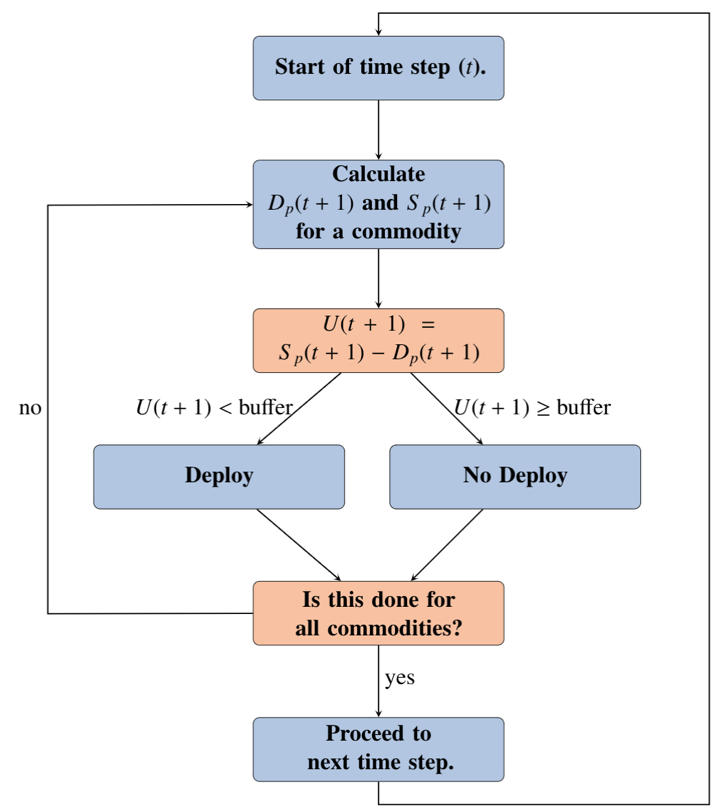
\includegraphics[height=5.5cm]{./images/d3ploy-flow}
      \end{center}
            \caption{\texttt{d3ploy} logic flow \cite{chee_demonstration_2019}}
      \label{fig:d3ploy-flow}
    \end{figure}
          \end{columns}
  \end{frame}

\begin{frame}
	\frametitle{Roberto Fairhurst: Transition Scenarios}
		\begin{columns}
		\column[t]{6cm}
		Current research interests:
		\begin{block}{D3ploy}
			\begin{itemize}
				\item Obtaining results for all the scenarios.
				\item Putting together final report.
			\end{itemize}
		\end{block}

        \begin{figure}[htbp!]
     	\begin{center}
				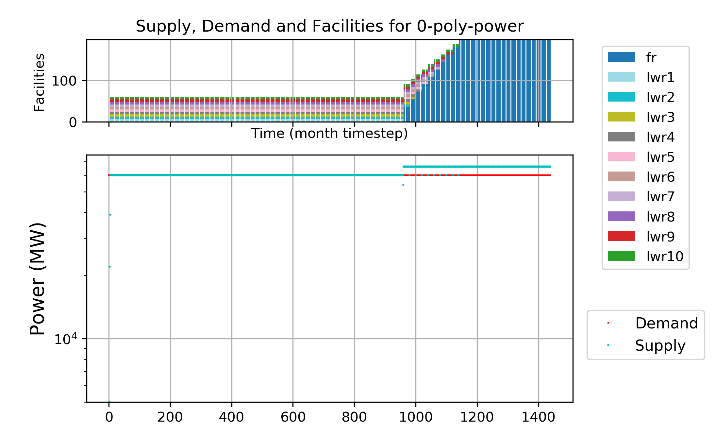
\includegraphics[height=3cm]{./images/eg23-power-poly}
			\end{center}
			\caption{Demand and supply of power for scenario eg01-eg23 using polynomial fit.}
			\label{fig:eg23-power}
	    \end{figure}

		\column[t]{4cm}
		\begin{figure}[htbp!]
			\begin{center}
				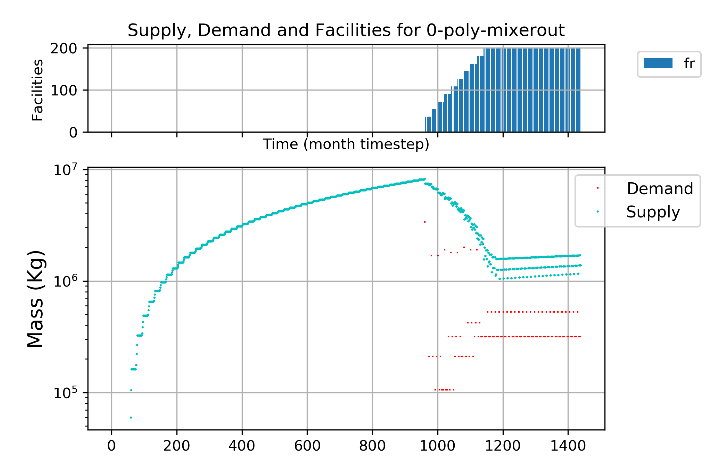
\includegraphics[height=3cm]{./images/eg23-frfuel}
			\end{center}
			\caption{Demand and supply of FR fuel for scenario eg01-eg23 using polynomial fit.}
			\label{fig:eg23-frfuel}
		\end{figure}
		\end{columns}
\end{frame}

\section{Acknowledgments}
\input{acks}
%%--------------------------------%%
%%--------------------------------%%
\begin{frame}[allowframebreaks]
  \frametitle{References}
  \bibliographystyle{plain}
  {\footnotesize \bibliography{2019-09-05-group.bib} }
\end{frame}

%%--------------------------------%%

% Examples 
% ARFC Team: Some good examples of how to use beamer are in this file.
% You can use this to guide the preparation of slides.
\input{example}


\end{document}

